\documentclass[../Text/00main.tex]{subfiles}
\graphicspath{{../}}

\begin{document}


% add average computation times??
% add a b c d e to the plots!!

\section{Validation}

\subsection{Large domain Çubuk}

\begin{figure}
    \centering
    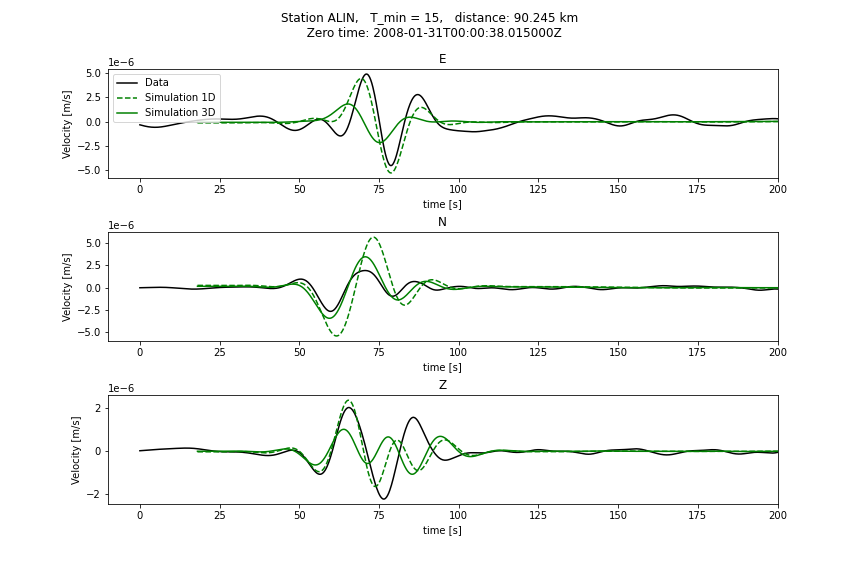
\includegraphics[width=0.5\linewidth]{images_results/KO.ALIN_15s_1D.png}
    \caption{Example of the comparison of 3D and 1D simulated velocity time series at station ALIN with the observed data. }
    \label{fig:ALINwv}
\end{figure}

A glance at examples of comparisons between data and the simulated signal filtered at $T = 15 s$ in Figure \ref{fig:ALINwv} (more in Appendix \ref{app:validation}) show that for the 3D model, the amplitudes generally match well, whereas the 1D model consistently over-estimates the amplitude. The start-time of the main waveform, and the duration of the signal after the main waveform is generally not reproduced accordingly by the simulation. 

\begin{figure}
    \centering
    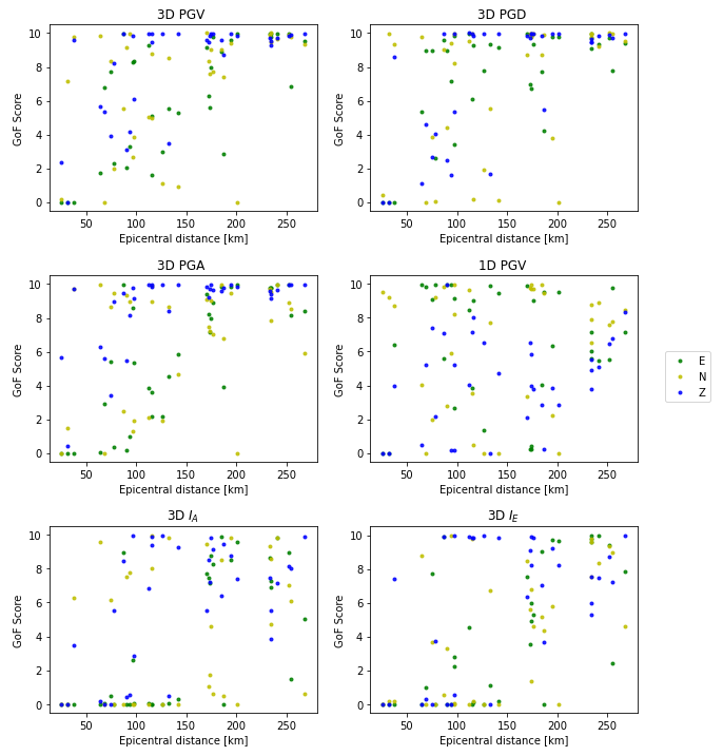
\includegraphics[width=.5\linewidth]{images_results/GOF_epicentral.png}
    \caption{Results of the large-domain PGA, PGV, PGD for the 3D model and PGV for the 1D model, as well as Arias intensity and the Energy integral. All data in E, N and Z direction with respect to epicentral distance.}
    \label{fig:gofpot_epicentral_large}
\end{figure}

 Figure \ref{fig:gofpot_epicentral_large} shows that the GoF of IMs is improving with epicentral distance for the peak-based parameters using a 3D model. This trend is especially strong with the Z-component. The 1D model shows a less clear improvement with epicentral distance. %iets over teleseismic distances??
 % move this?

% If you use beamer only pass "xcolor=table" option, i.e. 
%\documentclass[xcolor=table]{beamer}
\begin{table}[h!]
\caption{Table of the a selection of \cite{anderson_quantitative_nodate} GoF criteria for receivers in domain Çubuk\_L. Criterium C6b (red) was not taken into account for the total average score. }
\begin{tabular}{@{}l|llllll@{}}

\toprule
\textbf{Criterium} & \textbf{Parameter} & \textbf{Definition} & \textbf{E} & \textbf{N} & \textbf{Z} & \textbf{Average E,N,Z} \\ \midrule
\textbf{C3}            & Arias intensity &  & 3.77  & 4.33  & 5.87  & 4.65666667 \\
\textbf{C4}            & Energy integral &  & 4.24  & 4.23  & 6.03  & 4.83333333 \\
\textbf{C5}            & PGA             &  & 5.8   & 6.65  & 8.7   & 7.05       \\
\textbf{C6a}           & PGV 3D          &  & 6.37  & 6.89  & 8.12  & 7.12666667 \\
\textbf{C7}            & PGD             &  & 7.53  & 7.09  & 7.49  & 7.37       \\
\rowcolor[HTML]{FFCCC9} 
\textbf{C6b}           & PGV 1D          &  & 6.48  & 6.49  & 4.27  & 5.74666667 \\ \midrule
\textbf{Average score} &                 &  & 5.542 & 5.838 & 7.242 & 6.20733333 \\ \bottomrule
\end{tabular}
\label{tab:GoF_table_large_domain}
\end{table}

We evaluate the performance of this lower-frequency simulation basis of Andersons (ref) Goodness-of-fit criteria C2-C7. Mean scores per direction in table \ref{tab:GoF_table_large_domain} show that the peak-based parameters such as PGA, PGV and PGD perform well, with the majority of fits scoring in the good and excellent category. From the dPGV follows that the simulation generally produces higher peak amplitudes than the recorded data. This also is in agreement with further examination of the waveforms in Appendix \ref{app:validation}. The more duration-based Energy and Arias parameters score in the "poor" and "bad" fit categories, and do not show a clear trend with epicentral distance. This is to be expected, as the duration of the signal is not captured well by the simulation. % meeeer hier over!!! 

Spectral parameters such as the SA and SV were not considered for this lower-frequency simulation, as the maximum frequency only reaches the lowest frequency band. As peak-based parameters prove to be the more accurate intensity measures, further focus of this study  will be mainly on the PGV.

The spatial distribution of the GoF for the PGV in the large domain (Figure \ref{fig:gofmapsPGV_small} ) shows a clear trend of a better fit with distance. The over-all fit for the Z direction is better than the horizontal components. This is in line with the previous observations in the waveforms for 15 Hz. 

\section{Small domain}

To mitigate elevated computational costs, higher-frequency simulations for validation were conducted for this smaller sub-domain. Figure \ref{fig:gofmapsPGV_small} shows the overview of the varying waveform fits for the different stations in this domain.  

\hl{I'm not sure how to approach this. I have a very large collection of images of waveforms at periods from 20s - 1s, but only the 1Hz plots already take up a lot of space} Waveform results for $1 Hz$ in Figure \ref{fig:monsterfigurea} and \ref{fig:monsterfigureb} filtered at their respective minimum wavelengths, as well as their arias intensity and Ssa spectra, show that amplitudes are in good accordance with the observed data filtered at the same frequencies. The Arias intensity is under-estimated by the $1 Hz$ simulations. The fit of the 5\% damped Ssa varies per receiver, see Figure \ref{fig:GoFsevenstations} for the GoF of each evaluated parameter at $1 Hz$. 

\hl{Here I would like to implement the figure of GoF with increasing frequency.}
Supported by the GoFs in Figure \ref{fig:GoFsevenstations}, 

The timing, waveform similarity and duration however decrease with increasing frequency, as is to be expected with the simulation frequency surpassing the maximum resolution of the model. 

\begin{figure}
     \centering
     \begin{subfigure}{0.4\textwidth}
         \centering
         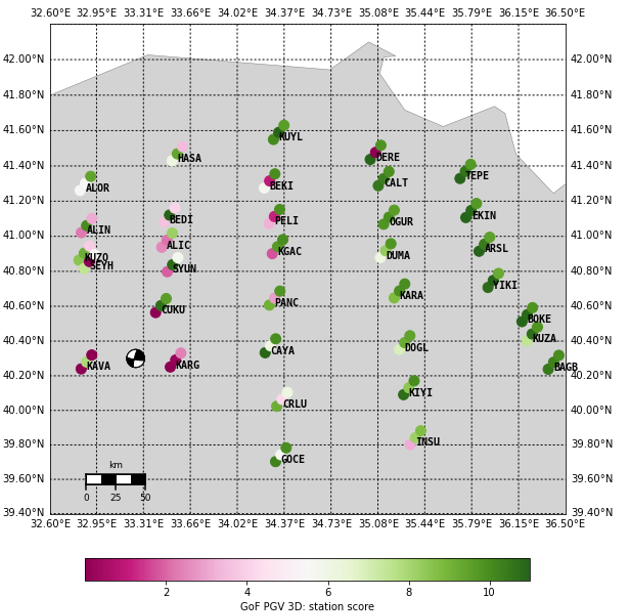
\includegraphics[width=\textwidth]{images_results/GoFmapPGV_large.png}
         %\caption{$y=x$}
         \label{fig:y equals x}
     \end{subfigure}
     \hfill
     \begin{subfigure}{0.4\textwidth}
         \centering
         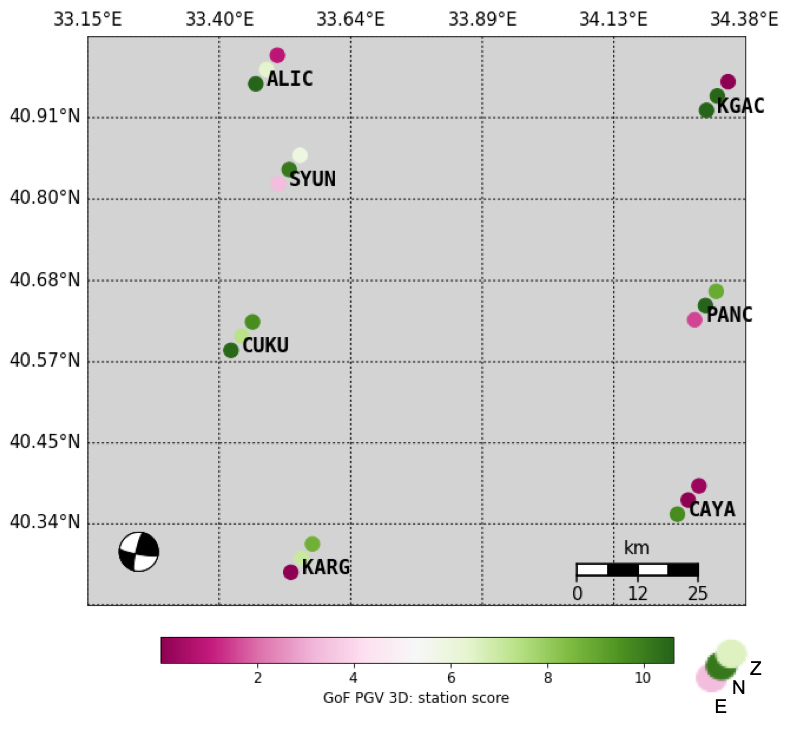
\includegraphics[width=\textwidth]{images_results/GoFmapPGV_smalle.png}
       
         \label{fig:three sin x}
     \end{subfigure}
     \caption{PGV goodness of fit for 15 Hz, per receiver in E (bottom), N(middle), and Z(top) directions. For the total domain on the left and the smaller sub-domain on the right.}
    \label{fig:gofmapsPGV_small}
\end{figure}



\begin{figure}
    \centering
    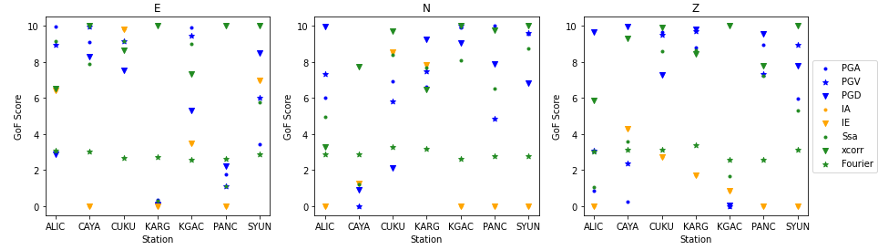
\includegraphics[width=\linewidth]{images_results/Gofsevenstations.png}
    \caption{Goodness of fit for the seven stations and all tested GoF parameters. \hl{Intend to change this for a figure that shows the change of fit with increasing frequency}}
    \label{fig:GoFsevenstations}
\end{figure}



\begin{sidewaysfigure}[!htp]
    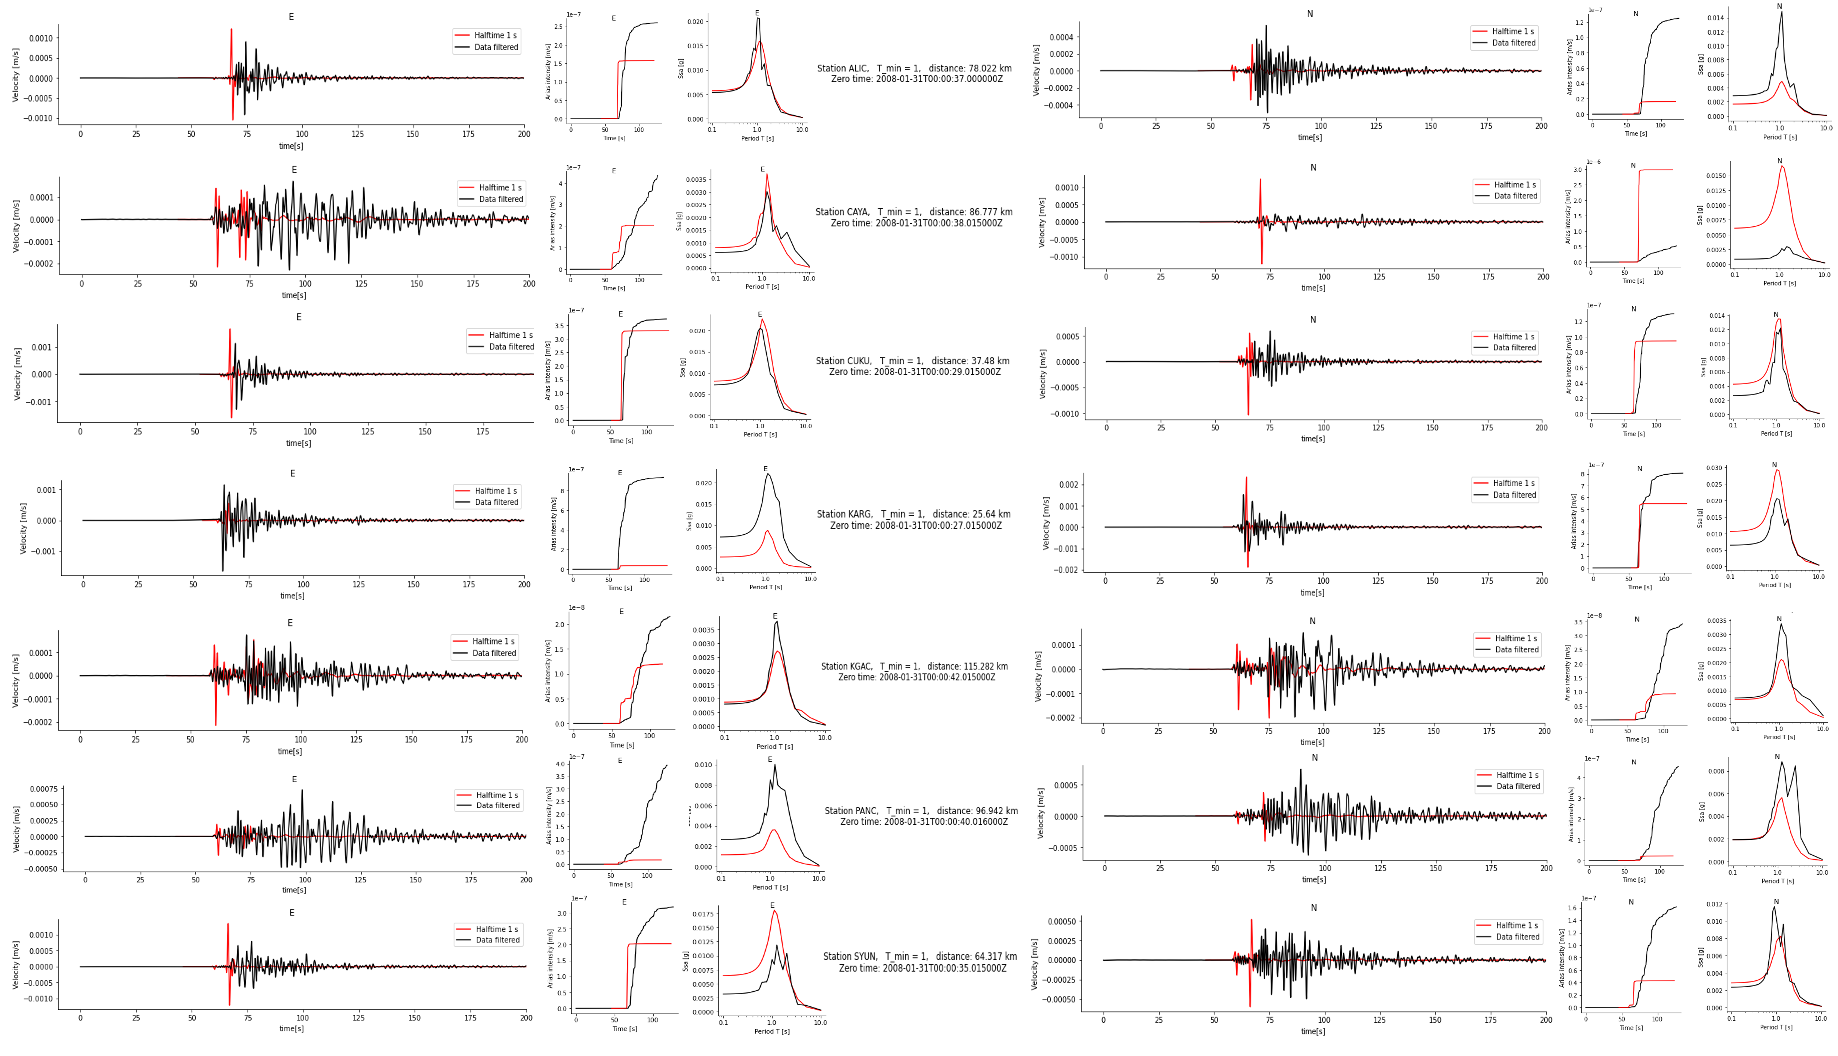
\includegraphics[width=\textwidth]{images_results/Monsterfigure_waveforms_pt1.png}
  \caption{Velocity time series, Arias intensities and pseudo-spectral accelerations for all seven receivers, filtered at 1Hz. }
  \label{fig:monsterfigurea}
\end{sidewaysfigure}


\begin{sidewaysfigure}[!htp]

    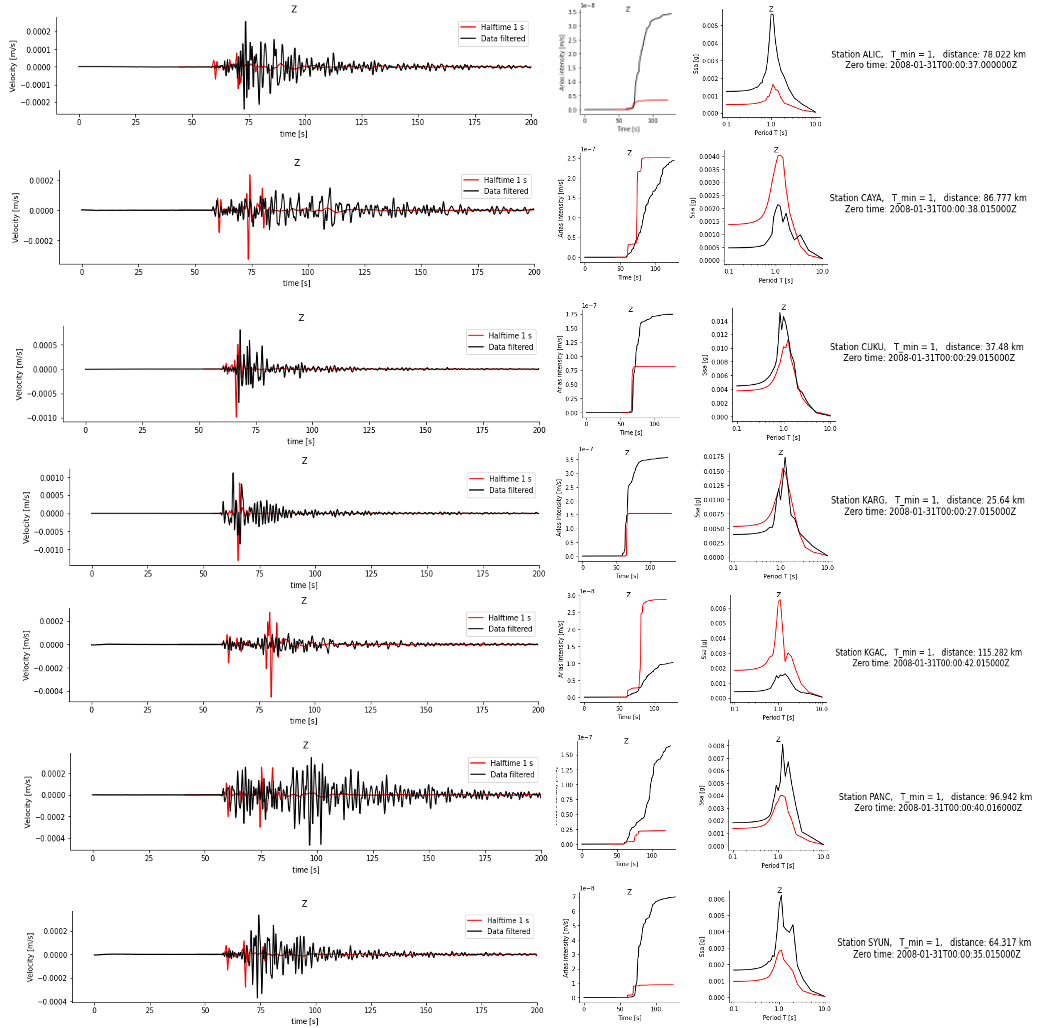
\includegraphics[width=0.6\textwidth]{images_results/monsterfigure_waveforms_pt2.png}
  \caption{Velocity time series, Arias intensities and pseudo-spectral accelerations for all seven receivers, filtered at 1Hz.}
  \label{fig:monsterfigureb}
\end{sidewaysfigure}

\FloatBarrier

\section{Reference scenario and domain complexity}




\subsection{CMT1, perfect strike-slip}

Here we present the results for an event with an artificial magnitude of $M_0 = 1.0$. The reference event CMT1 consists of a perfect strike-slip source with strike, dip and rake as 90, 90, 180 (see Table \ref{tab:CMTstarts}). In this section, the differences between the reference event for the four proposed scenarios (1D, 3D, 3D + topo, 3D + topo + ocean) are evaluated and compared to the results of the 3D domain. 

Figure \ref{fig:ref_CMT1} shows the PGV distribution of the event for the E, N and Z orientations in the four domain types. Results are normalised over the 3D scenario in each direction. 

\begin{figure}[htp!]
    \centering
    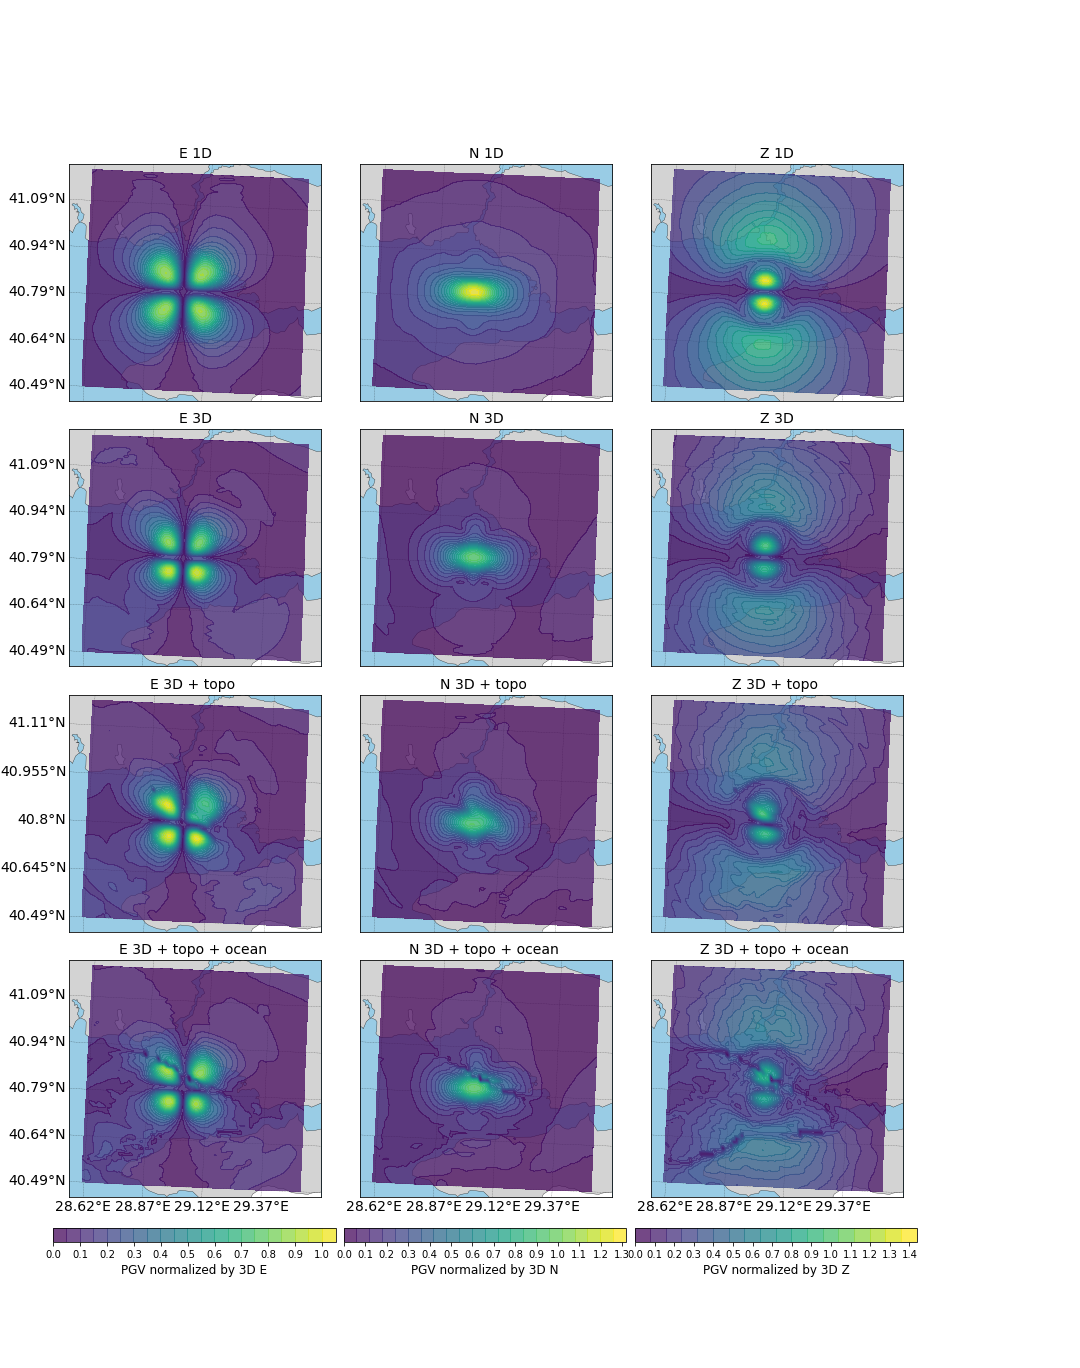
\includegraphics[width=1.2\linewidth]{images_results/Ref_scenarios_normalized_sc1.png}
    \caption{PGV reference scenario CMT1, strike 90, dip 90, rake 180, normalized with respect to the 3D configuration (top row).}
    \label{fig:ref_CMT1}
\end{figure}

\subsubsection{3D}

In this reference scenario, we see a very clear pattern of the peak ground velocity that the perfect strike-slip mechanism has produced. Where the source imprint on the pattern is strong close to the source, it is more influenced by the complexities of the model in the far field.

\subsubsection{1D}

The result of the spatial distribution of the PGV in the 1D domain is similar to the 3D result, and could be seen as a smoothed version of the 3D model result. Its peak PGV is intensified especially in the North and Z direction. This is in line with the results in the validation phase, where the 1D model consistently over-estimates the 3D model. 

\subsubsection{3D + topography}

Topography has distorted the clear pattern as seen in the flat domains, especially along the steep ridge to the North-East of the source location. This effect is more strong in the horizontal directions than in the Z-direction. The PGV is amplified in the E and Z direction, and slightly de-amplified in the N direction. The influence on the far field is not very strong. 

\subsubsection{3D + topography + ocean}

The immediate observation in this pattern is the influence of the mesh deformation where the simulated water layer stops and the ocean loading starts. Especially to the North-East of the source location, this effect is strong. The steep topography causing effects in the 3D + topography set-up is coinciding here with the change of ocean solid-fluid coupling and ocean loading.

\begin{figure}[htp!]
    \centering
    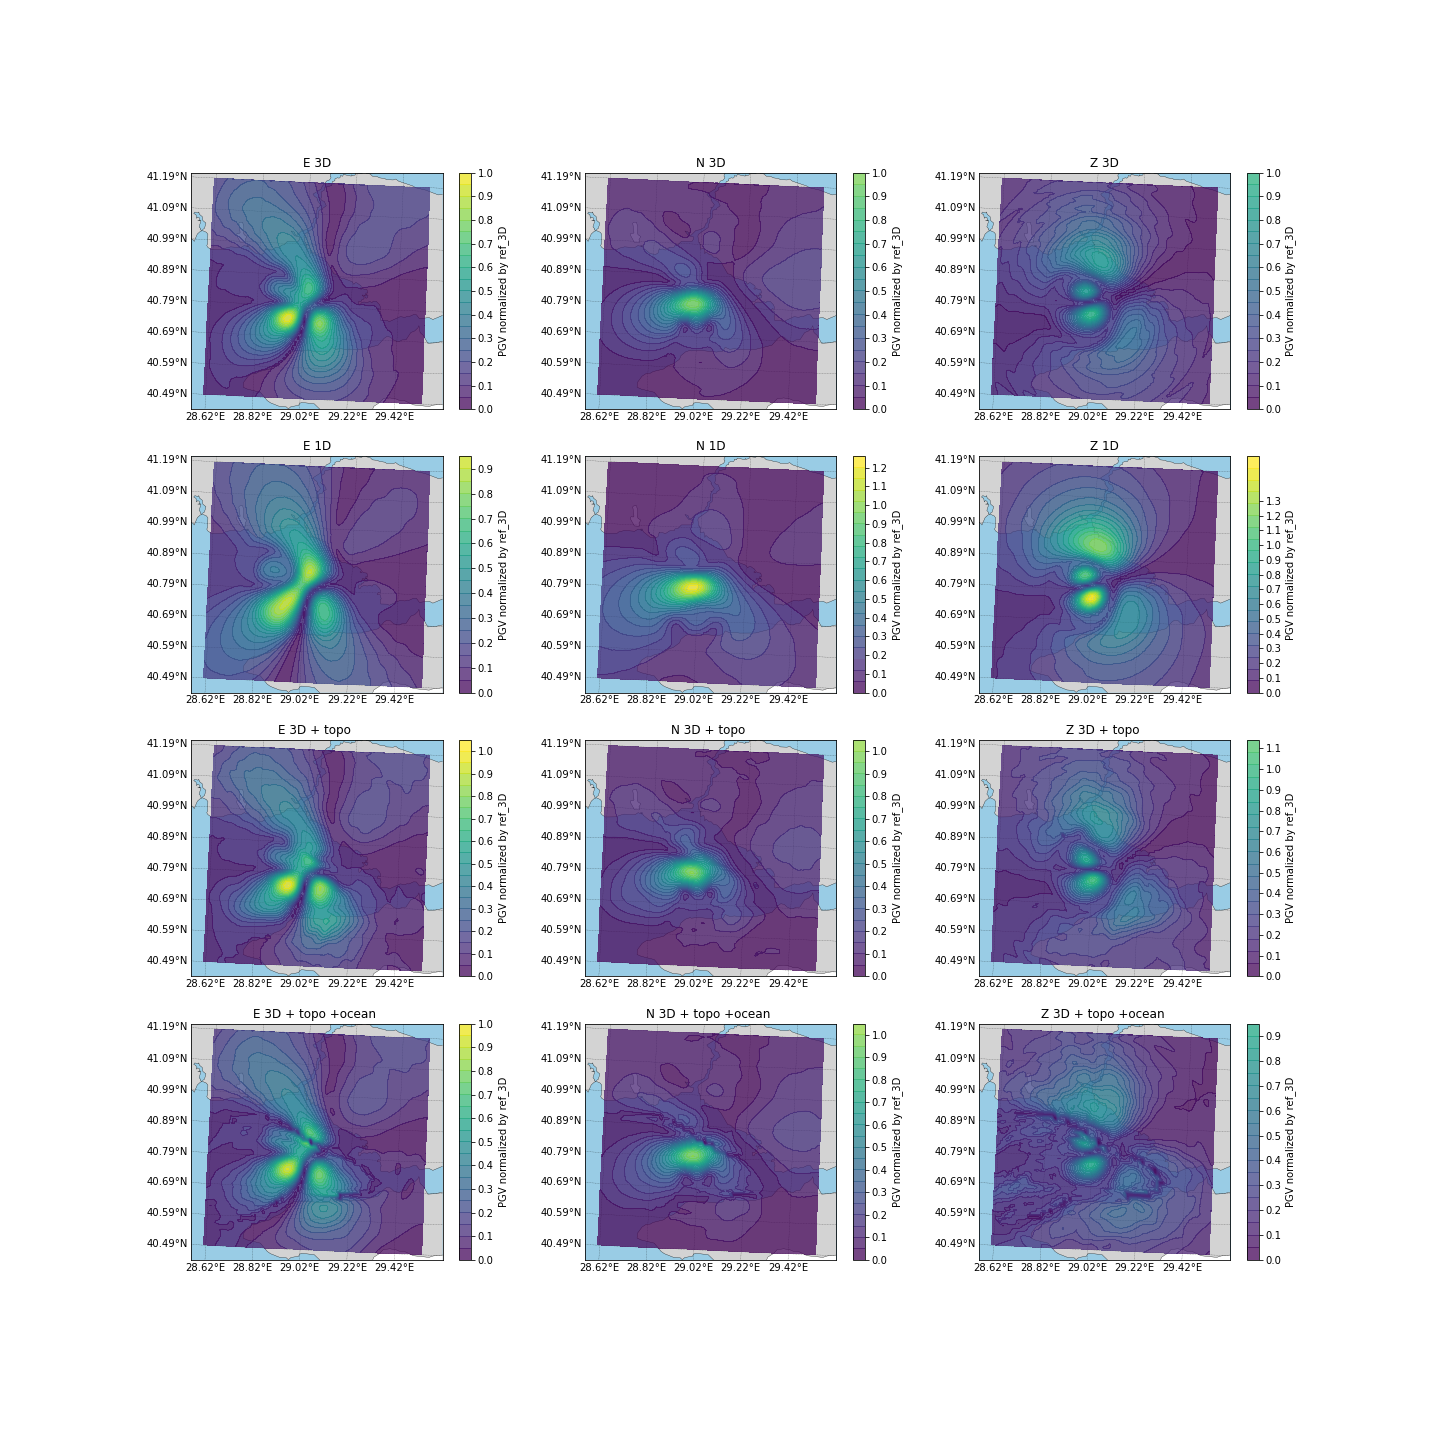
\includegraphics[width=1.2\linewidth]{images_results/Ref_scenarios_normalized_sc2.png}
    \caption{PGV reference scenario CMT2, strike 100, dip 75, rake 160, normalized with respect to the 3D configuration (top row).}
    \label{fig:ref_CMT2}
\end{figure}

\subsection{CMT2 strike-slip}

Another strike-slip scenario, now with a slightly tilted strike (90 $\degree$), a less steep dip (75 $\degree$) and a rake that indicates a slightly more oblique faulting mechanism (160 $\degree$). The main motivation for this is to remain in a regime that is realistic for the NAFZ, but starts from a starting point that does not involve fractions of $\frac{\pi}{2}$, to avoid zeros in the moment tensor components. 

\hl{To do this needs more (visual) explanation. I will add a figure in appendix}

\subsubsection{3D}

% add the differences between the larges PGV in 3 directions.

The strike-slip pattern is now slightly at an angle, and has a stronger PGV in the slip direction of the hanging wall to the South-West of the source. 

\subsubsection{1D}

The 1D model pattern is again a smoothed version of the 3D PGV pattern. It ignificantly amplifies the velocities in the N and Z directions by over 20\%. However, the pattern remains very similar to the 3D scenario. 

\subsubsection{3D + topo}

The topography causes  distortion of the PGV pattern once again to the North-East of the source. It focuses slightly more energy towards the source zone. 

\subsubsection{3D + topo + ocean}

The imprint of the edge of the fluid-solid coupling is again very visible in the PGV pattern. Other than that, it is not significantly different from the PGV pattern of the 3D + topo scenario.

\subsection{More CMT starting configurations}

Even though the fault at question is characterised as a strike-slip fault, we have tested two other scenarios: CMT3 and CMT4 (see Table \ref{tab:CMTstarts}). These other two starting configurations comprise a normal (CMT3) and thrust (CMT4) regime. The motivation behind this was to test whether the effects observed were unique to a strike-slip configuration, or if these observations could be consistent for other types of faulting. The resulting images of these two configurations are displayed in Appendix \ref{app:morereffigs}.

%An overview of the four domain types for the reference scenario is given in Figure (\hl{paraview image of four domain types?}). 

\FloatBarrier

\section{Moment tensor component variation}

In this section we deviate from the CMT starting configurations as stated in Table \ref{tab:CMTstarts}. 

\subsection{strike}

\subsubsection{CMT1}

\begin{figure}[!htb]
    \centering
    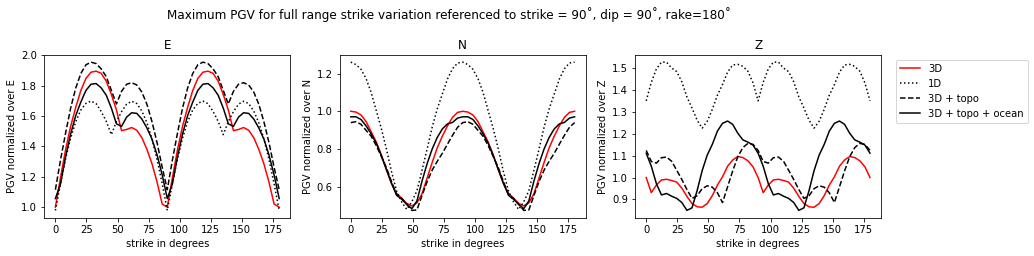
\includegraphics[width=0.8\textwidth]{images_results/fullrange1_strikevar_maxvals.png}
    \caption{Full 180$\degree$ range variation of the strike measured at station KAVV.}
    \label{fig:KAVV_fullrange_1}
\end{figure}

The strike has a range of 0 to 180$\degree$ total. It is varied here for 45$\degree$ in each direction. Figure \ref{fig:ref_sigma1_strike} shows the coefficient of variation $Cv$ with respect to each domain and starting scenario. E.g. for PGV N 3D + topo, the coefficient of variation is calculated with respect to the values of the reference scenario of PGV N 3D + topo. For the E and Z directions, the main and largest peak velocity variations take place along the initial strike of the fault. The north component shows a stronger variation near the +/- 45$\degree$ strike end-members of the variation. The 1D model in this case tells a very different story than the 3D models. It shows very symmetrical patterns compared to the simulations that made use of the 3D model. The lateral variations in the velocity model seem to cause more variation in the North-West section of the grid. The topography in the 3D + topo and 3D + topo + ocean scenarios has a damping effect on the velocity variations in the N and Z directions especially. The E direction for these scenarios shows a slightly perturbed result of the 3D model. The direct imprint of the edge of ocean coupling is less visible in this case and seems to have little influence on the variations. 

\begin{figure}[htb]
    \centering
    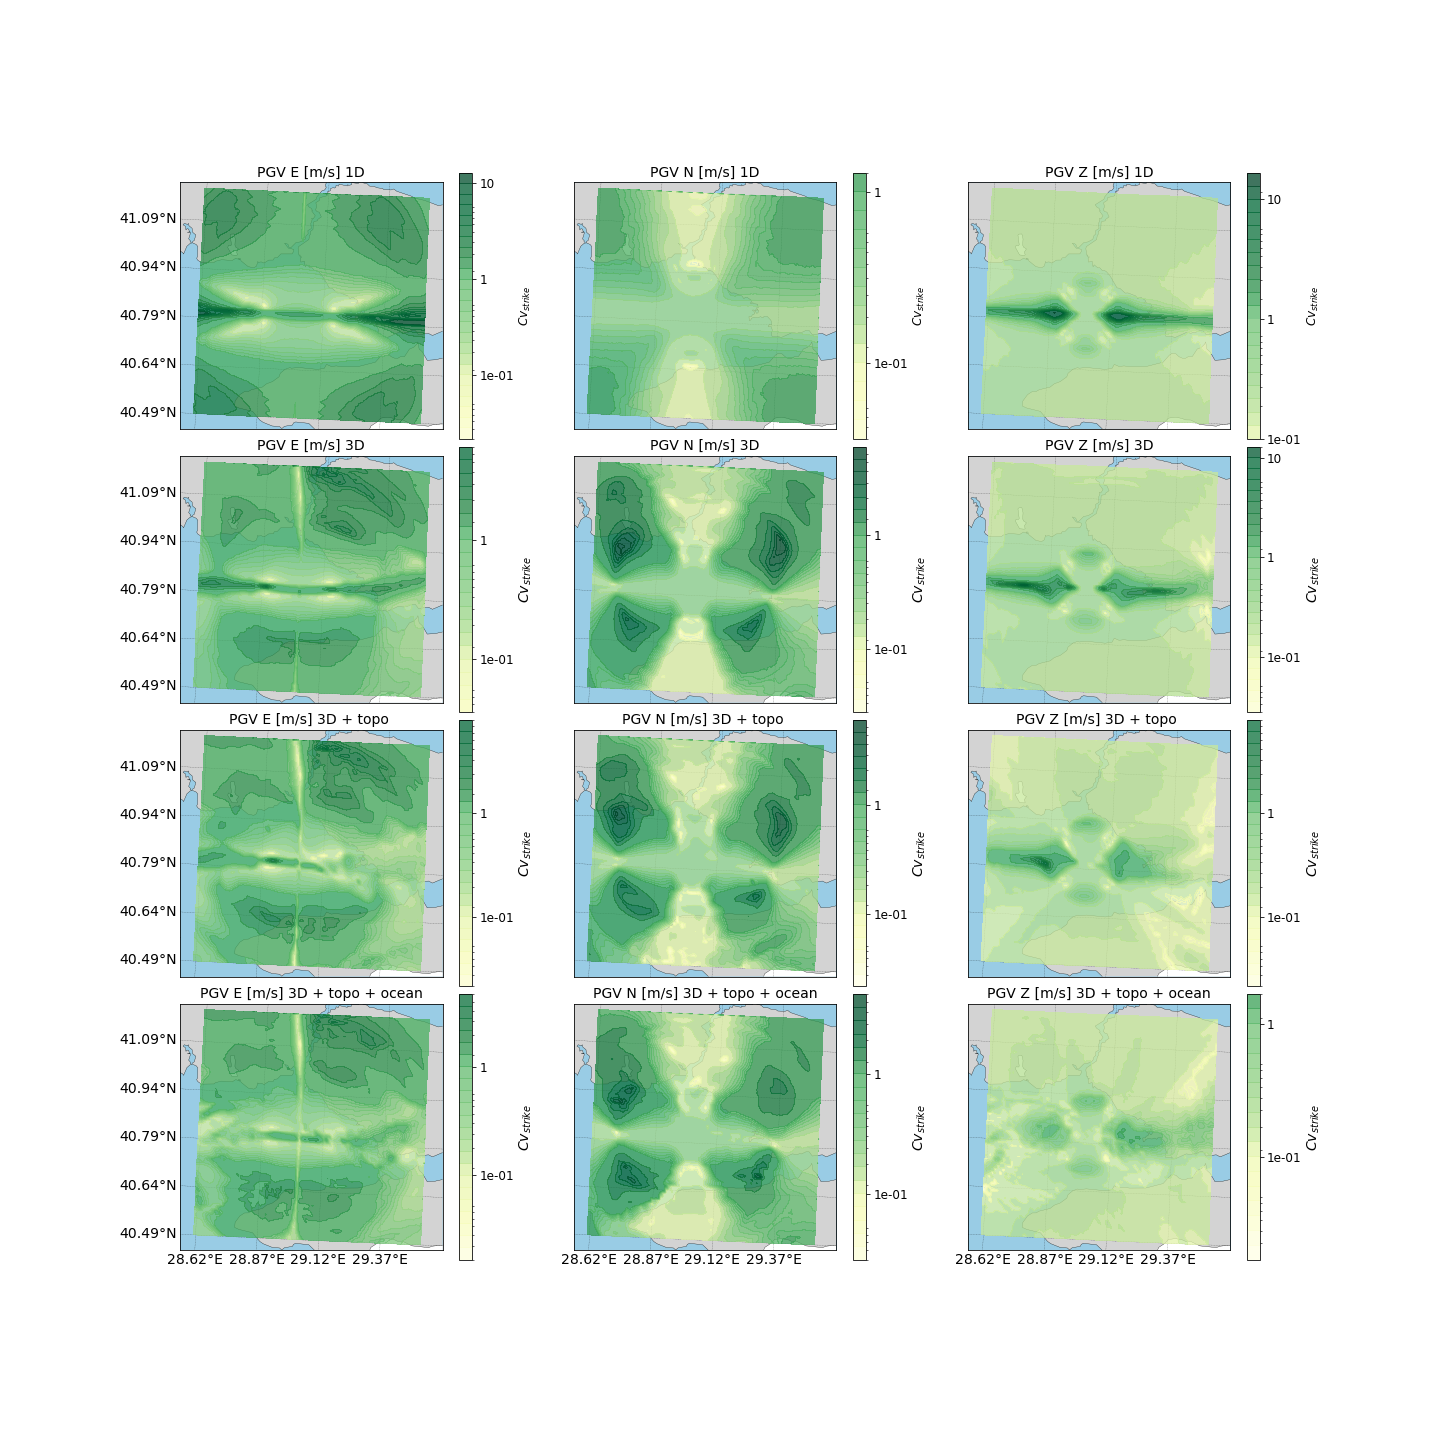
\includegraphics[width=1.2\linewidth]{images_results/strike_variation_sigma_sc1.png}
    \caption{CMT1 coefficient of variation $Cv$ of strike variation, for each model domain in E, N and Z direction. Colourbar set to logarithmic to adequately show the large differences.}
    \label{fig:ref_sigma1_strike}
\end{figure}


% check ff of dit klopt of het KAVV is

Figures \ref{fig:ref_eps12-1} and \ref{fig:ref_eps25-1} show the relative difference between the strike varied $- 15\degree$ and $- 22.5\degree$, respectively. Striking here is that relative difference does not change so much in pattern, as in intensity. Double the amount of variation seems to roughly double the relative difference at each point. The normalised full range of strike variation measured at station KAVV (Figure \ref{fig:KAVV_fullrange_1}) shows how the PGV varies with a strike that varies 180$\degree$. This periodic pattern supports that mainly the 1D pattern is exhibiting much higher peak velocities in N and Z directions at this point. The other scenarios are all in close range to each other. The 1D pattern here is more symmetrical, which could be attributed to the lack of lateral variations int he velocity model. Topography and ocean seem to have an influence mainly on the E and Z directions. 

\begin{figure}[!htb]
    \centering
    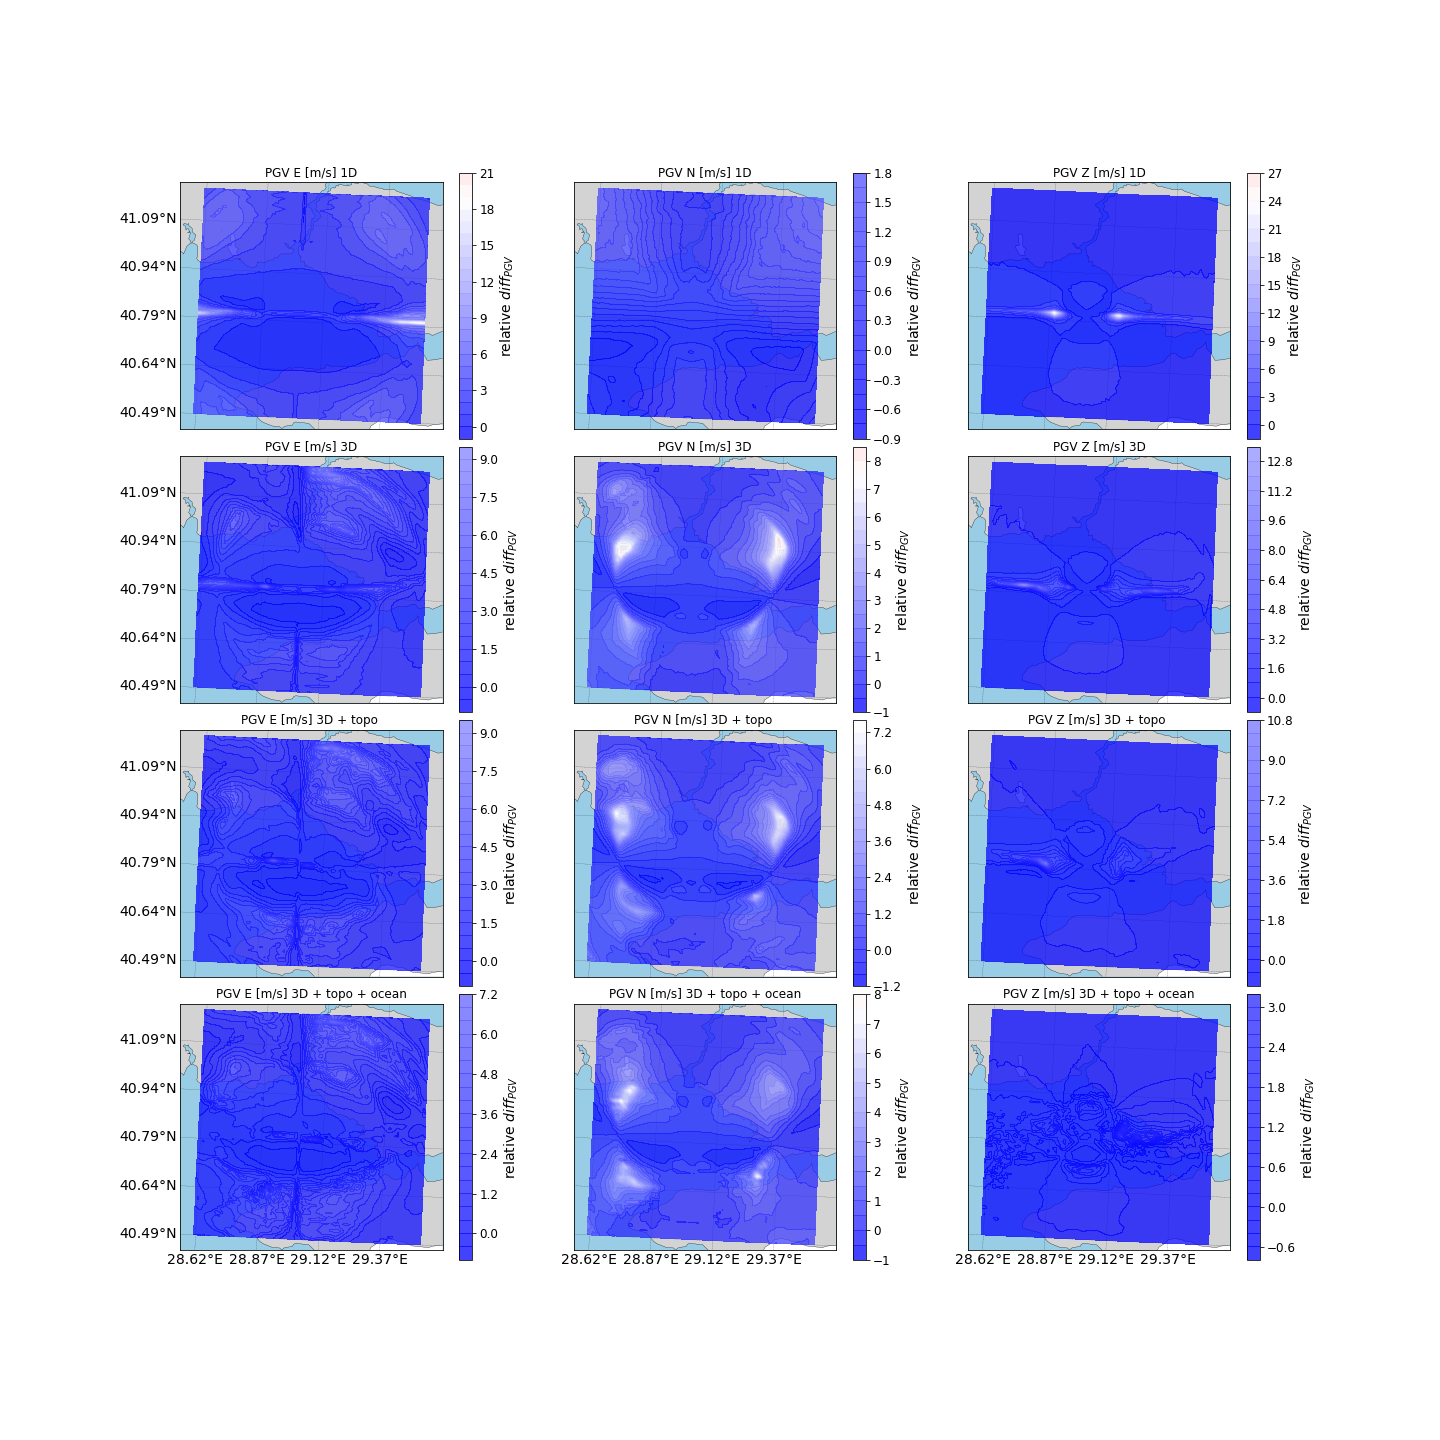
\includegraphics[width=1.2\linewidth]{images_results/strike_variation_epsilon12_sc1.png}
    \caption{CMT1 relative difference between a scenario with a strike variation of 15$\degree$ with respect to the reference scenario. Colorbar set to the total minima and maxima of the 15$\degree$ and 25$\degree$ plots for comparison.}
    \label{fig:ref_eps12-1}
\end{figure}

\begin{figure}[h]
    \centering
    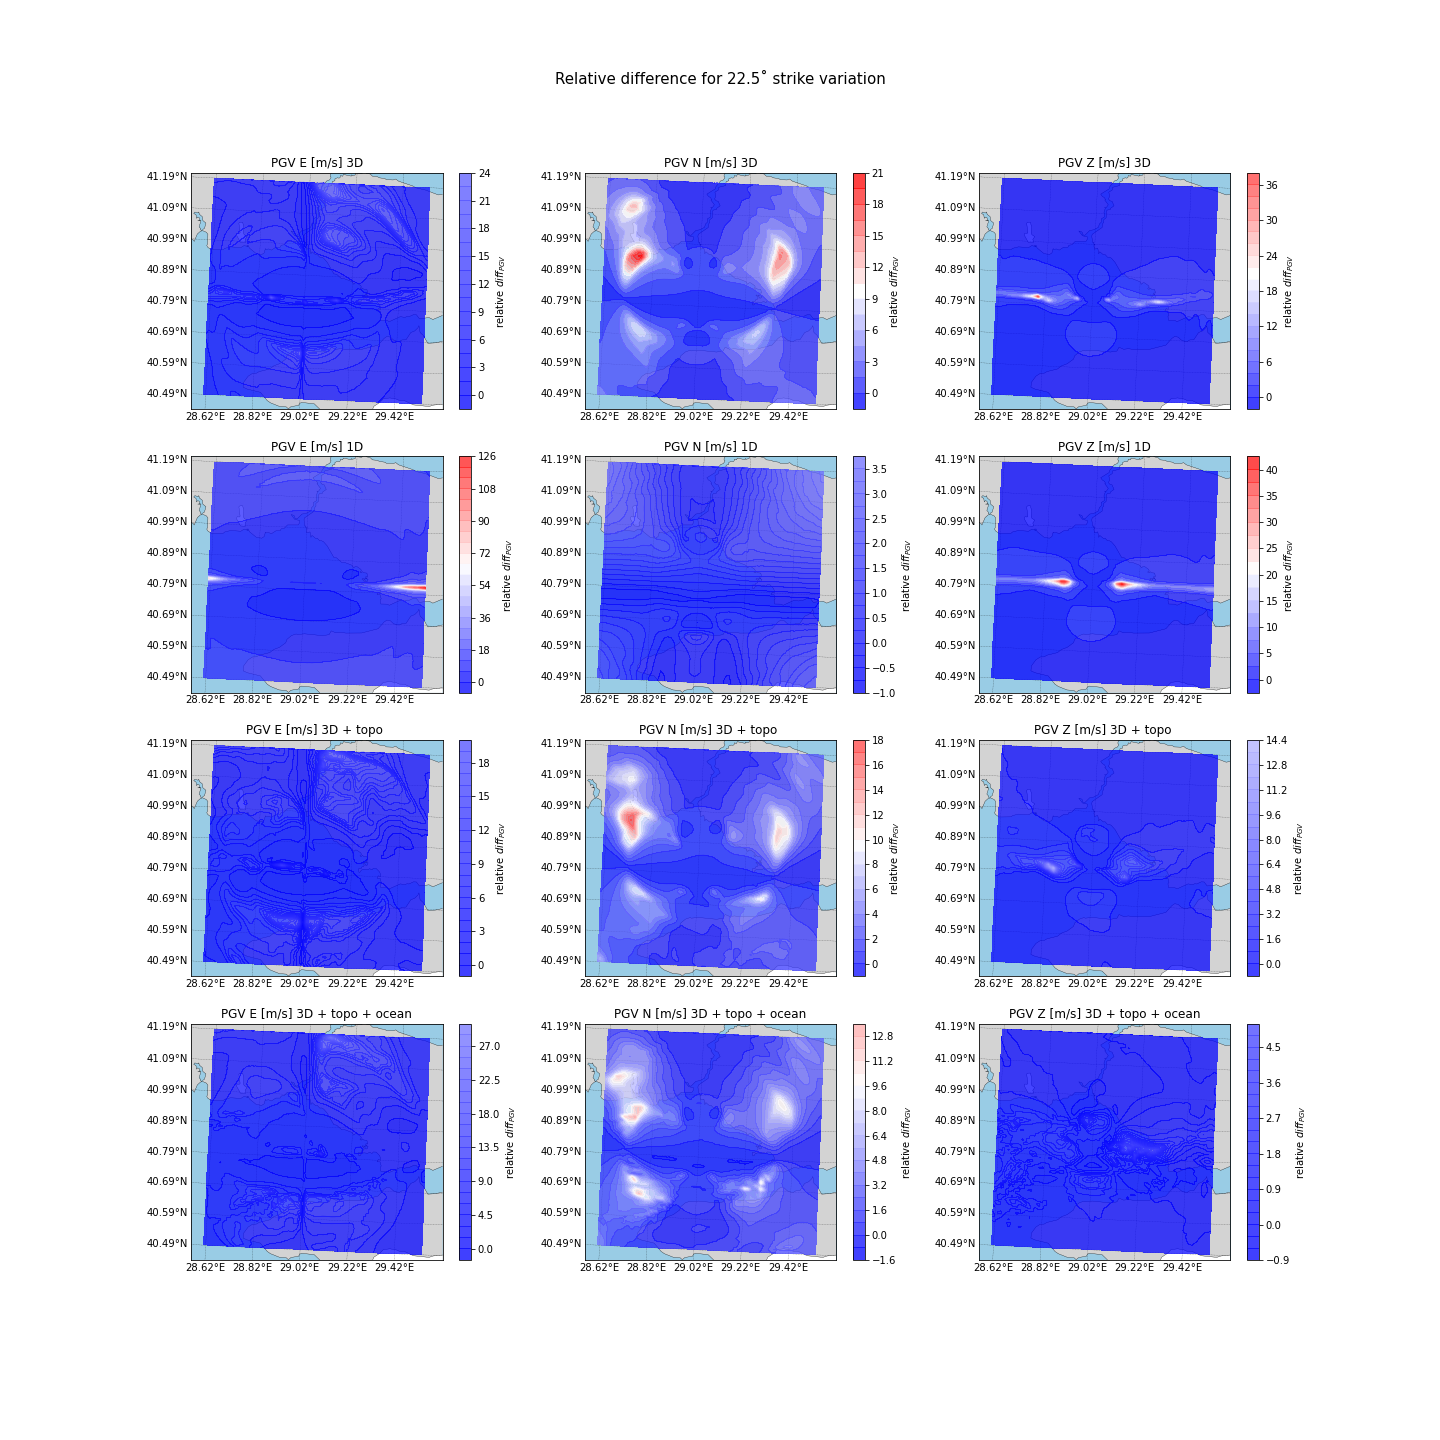
\includegraphics[width=1.2\linewidth]{images_results/strike_variation_epsilon25_sc1.png}
    \caption{CMT1 relative difference between a scenario with a strike variation of 25$\degree$ with respect to the reference scenario. Colorbar set to the total minima and maxima of the 15$\degree$ and 25$\degree$ plots for comparison.}
    \label{fig:ref_eps25-1}
\end{figure}

\FloatBarrier

\subsubsection{CMT2}

\begin{figure}[!htp]
    \centering
    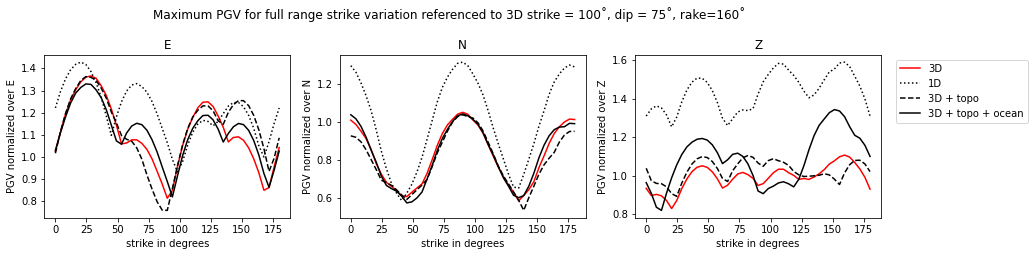
\includegraphics[width=0.8\textwidth]{images_results/fullrange2_strikevar_maxvals_sc2.png}
    \caption{CMT2 Full 180$\degree$ range variation of the strike measured at station KAVV.}
    \label{fig:KAVV_fullrange_2}
\end{figure}

The same is evaluated for the CMT2 starting configuration. The $Cv$ in Figure \ref{fig:cmt2sigm} now shows less symmetrical patterns than the simple CMT1 starting case. This could be attributed to the different dip and rake starting point, which alter the variation of the total moment tensor (\hl{To do: supporting figure in methods for strike/dip/rake variations and influence on the total moment tensor}). The same trends as in CMT1 with respect to de-amplification of the variation influence in the 3D + topo and 3D + topo + ocean scenarios can be observed. The doubling of relative difference between the 15$\degree$ varied and 25$\degree$ varied strike still holds here. The full range in Figure \ref{fig:KAVV_fullrange_2} shows the same trend as CMT1: the 3D models are in similar ranges, the 1D shows higher peak velocity.

\begin{figure}[!htp]
    \centering
    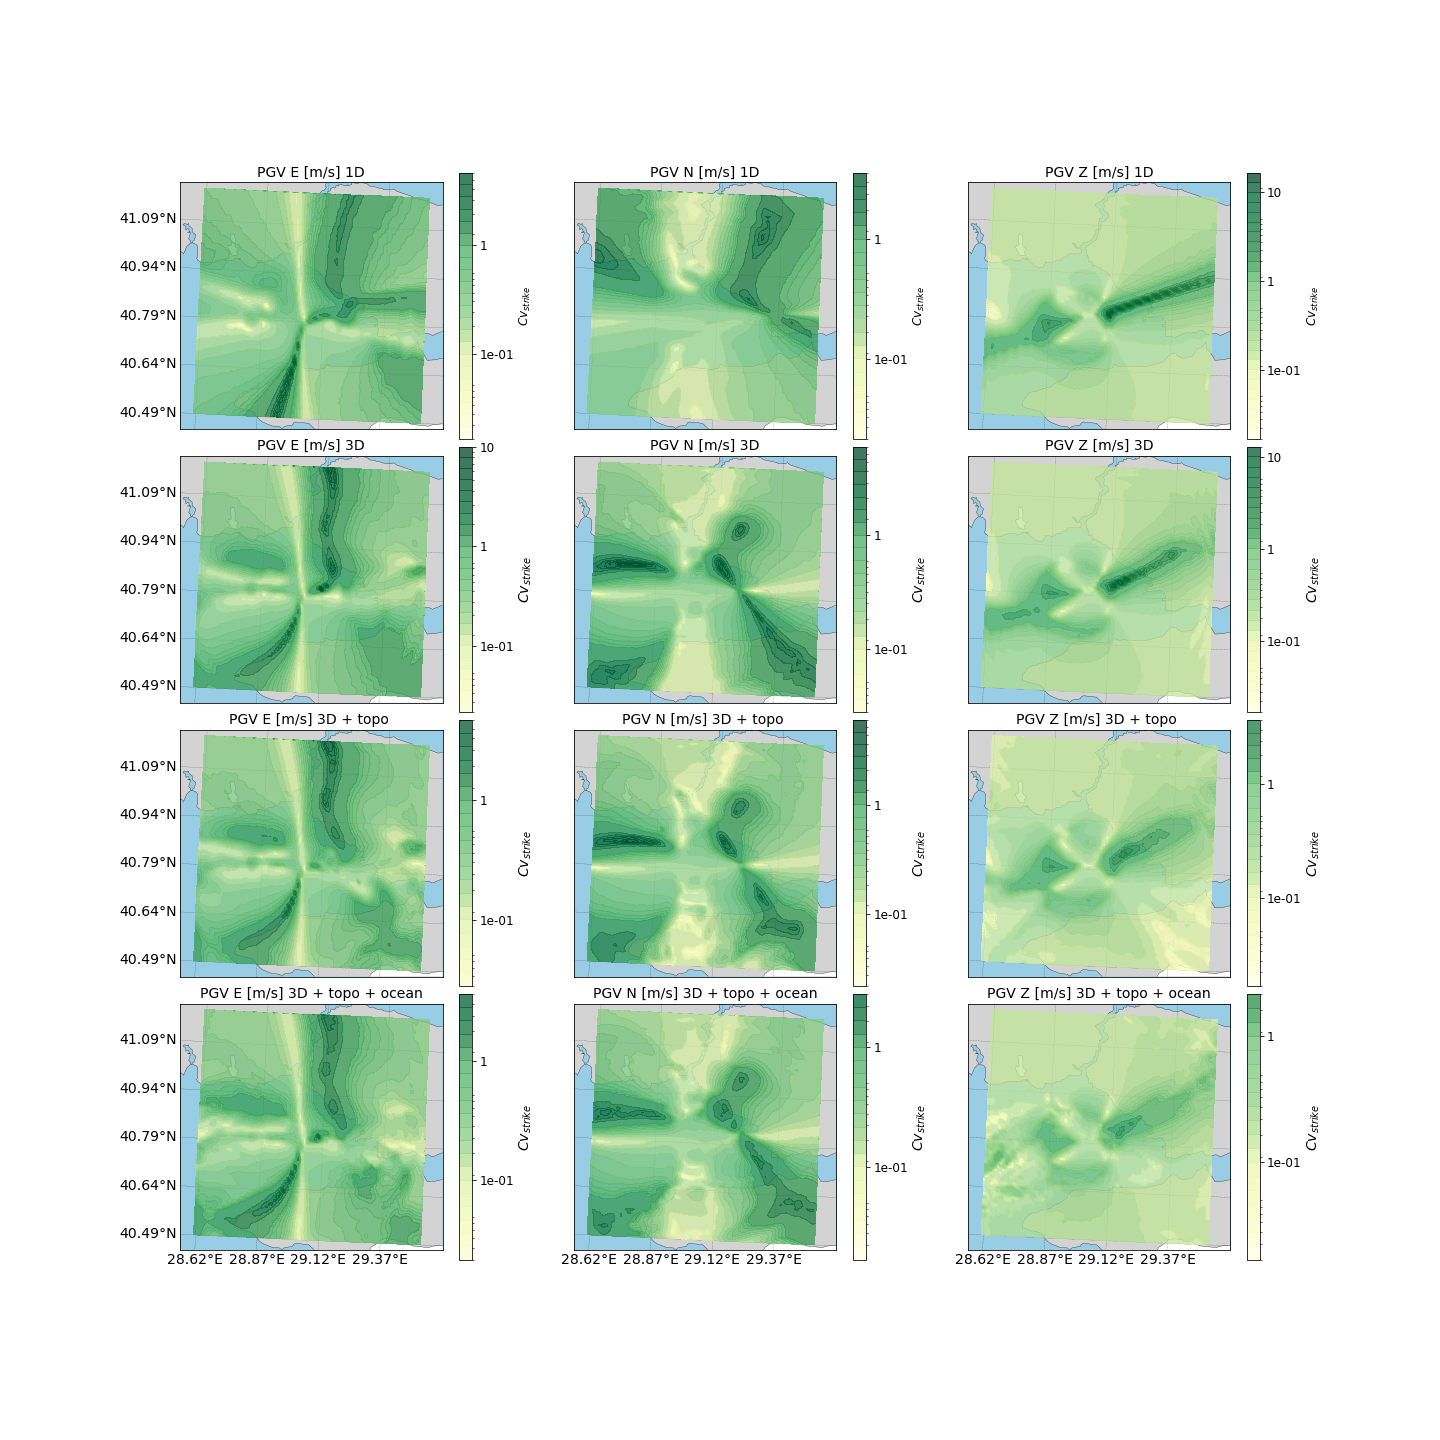
\includegraphics[width=1.2\linewidth]{images_results/strike_variation_sigma_sc2.png}
    \caption{CMT2 coefficient of variation $Cv$ of strike variation, for each model domain in E, N and Z direction. Colourbar set to logarithmic to adequately show the large differences.}
    \label{fig:cmt2sigm}
\end{figure}



\begin{figure}[!htp]
    \centering
    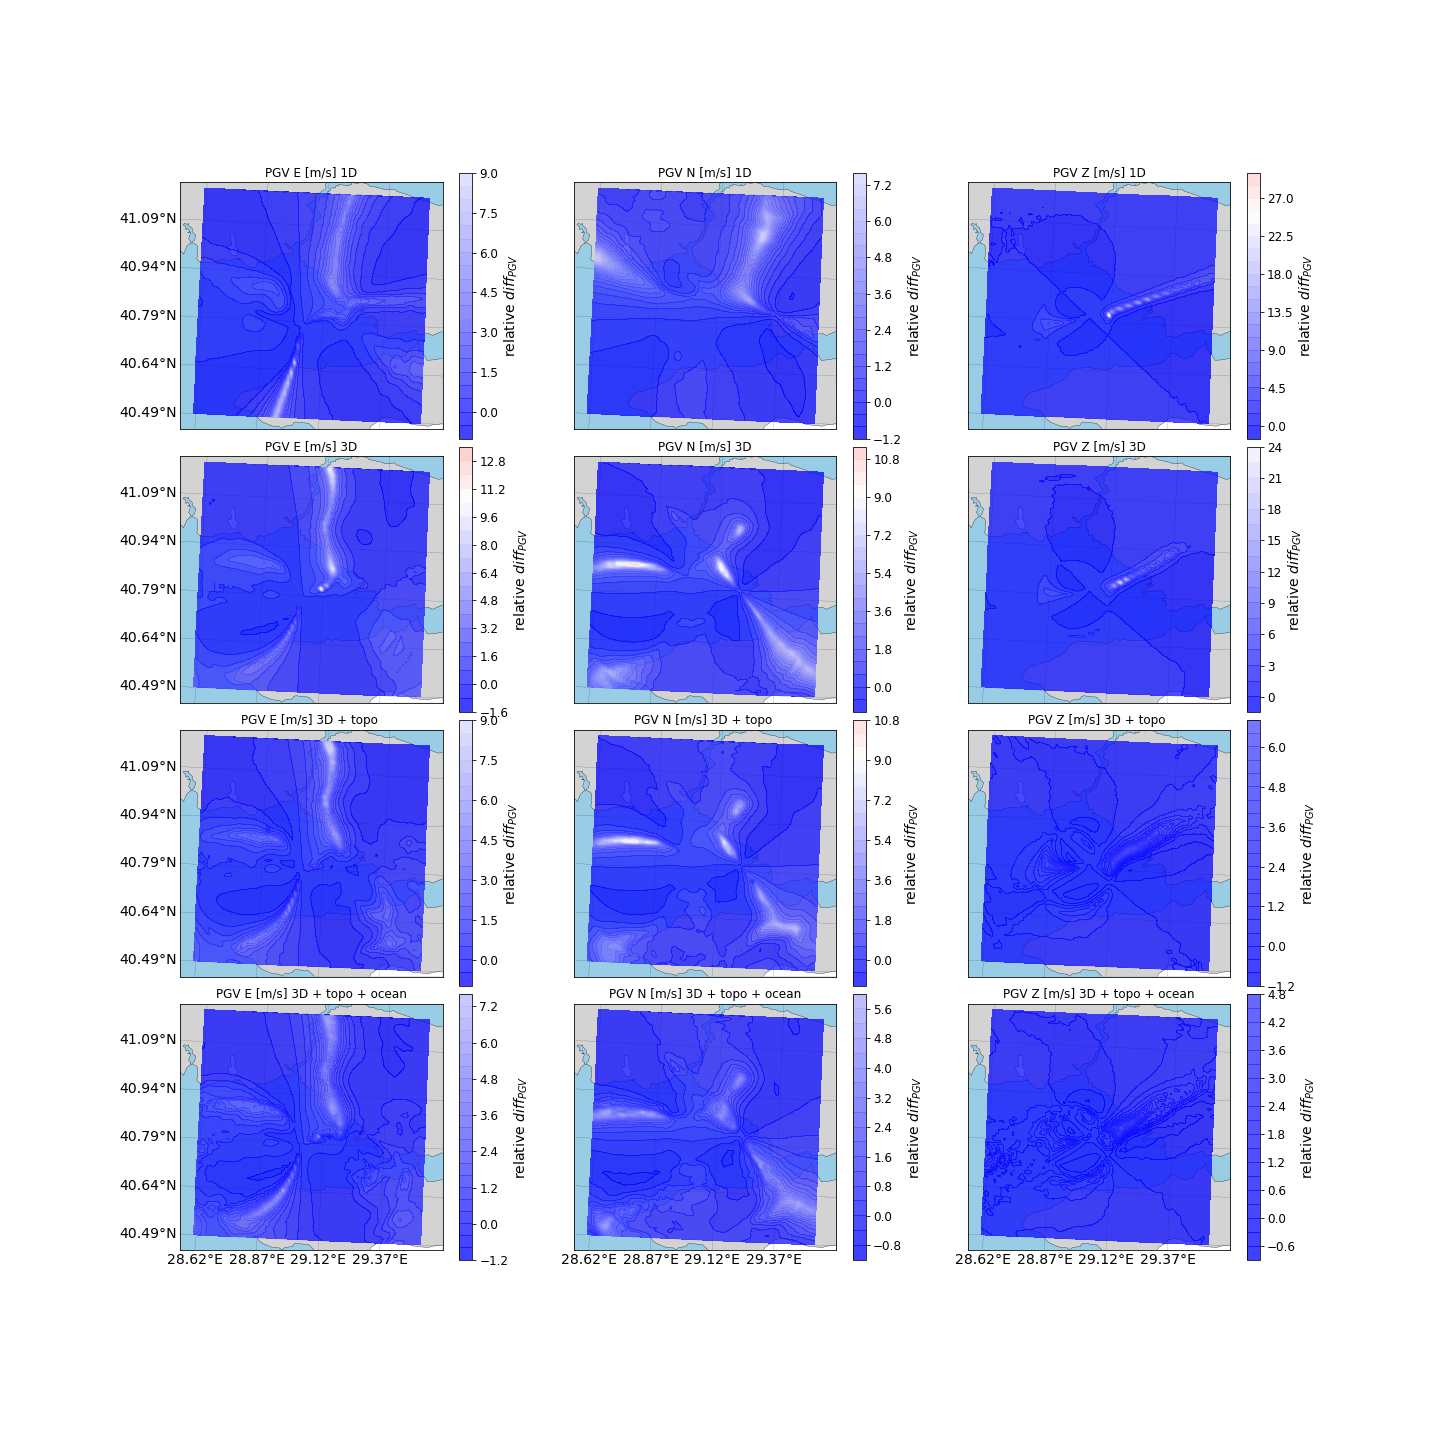
\includegraphics[width=1.2\linewidth]{images_results/strike_variation_epsilon12_sc2.png}
    \caption{CMT2 relative difference between a scenario with a strike variation of 15$\degree$ with respect to the reference scenario. Colorbar set to the total minima and maxima of the 15$\degree$ and 25$\degree$ plots for comparison.}
    \label{fig:ref_eps12-2}
\end{figure}

\begin{figure}[!htp]
    \centering
    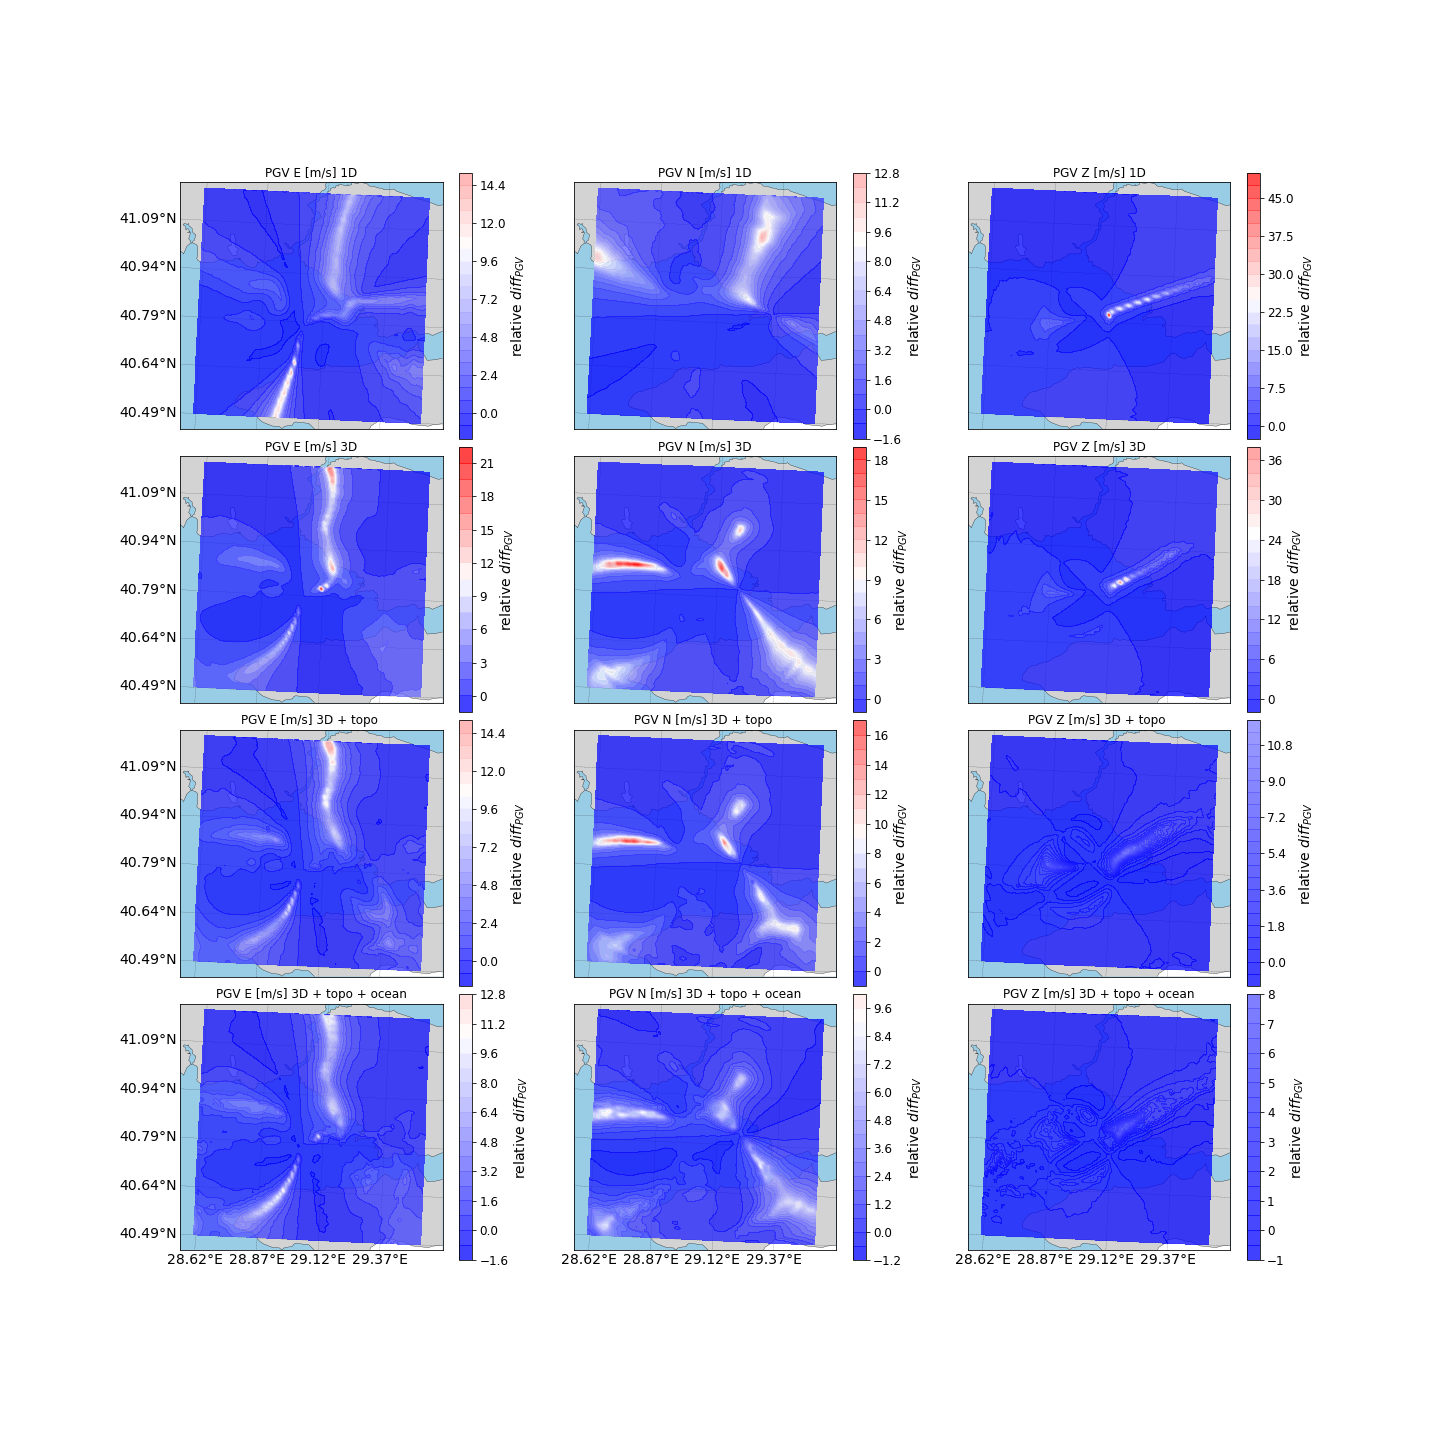
\includegraphics[width=1.2\linewidth]{images_results/strike_variation_epsilon25_sc2.png}
    \caption{CMT2 relative difference between a scenario with a strike variation of 25$\degree$ with respect to the reference scenario. Colorbar set to the total minima and maxima of the 15$\degree$ and 25$\degree$ plots for comparison.}
    \label{fig:ref_eps25-2}
\end{figure}

\FloatBarrier

%%%%%%%%%%%%%%%%%%%%%%%%%%%%%%
\subsection{dip}

\hl{repeat for dip and rake. I have found plotting mistakes here which I will fix first. Essentially, the same happens here with intensification of the pattern.}

% We vary the dip 45$\degree$ up-dip here. 

% \subsubsection{CMT1}

% \begin{figure}[htb]
%     \centering
%     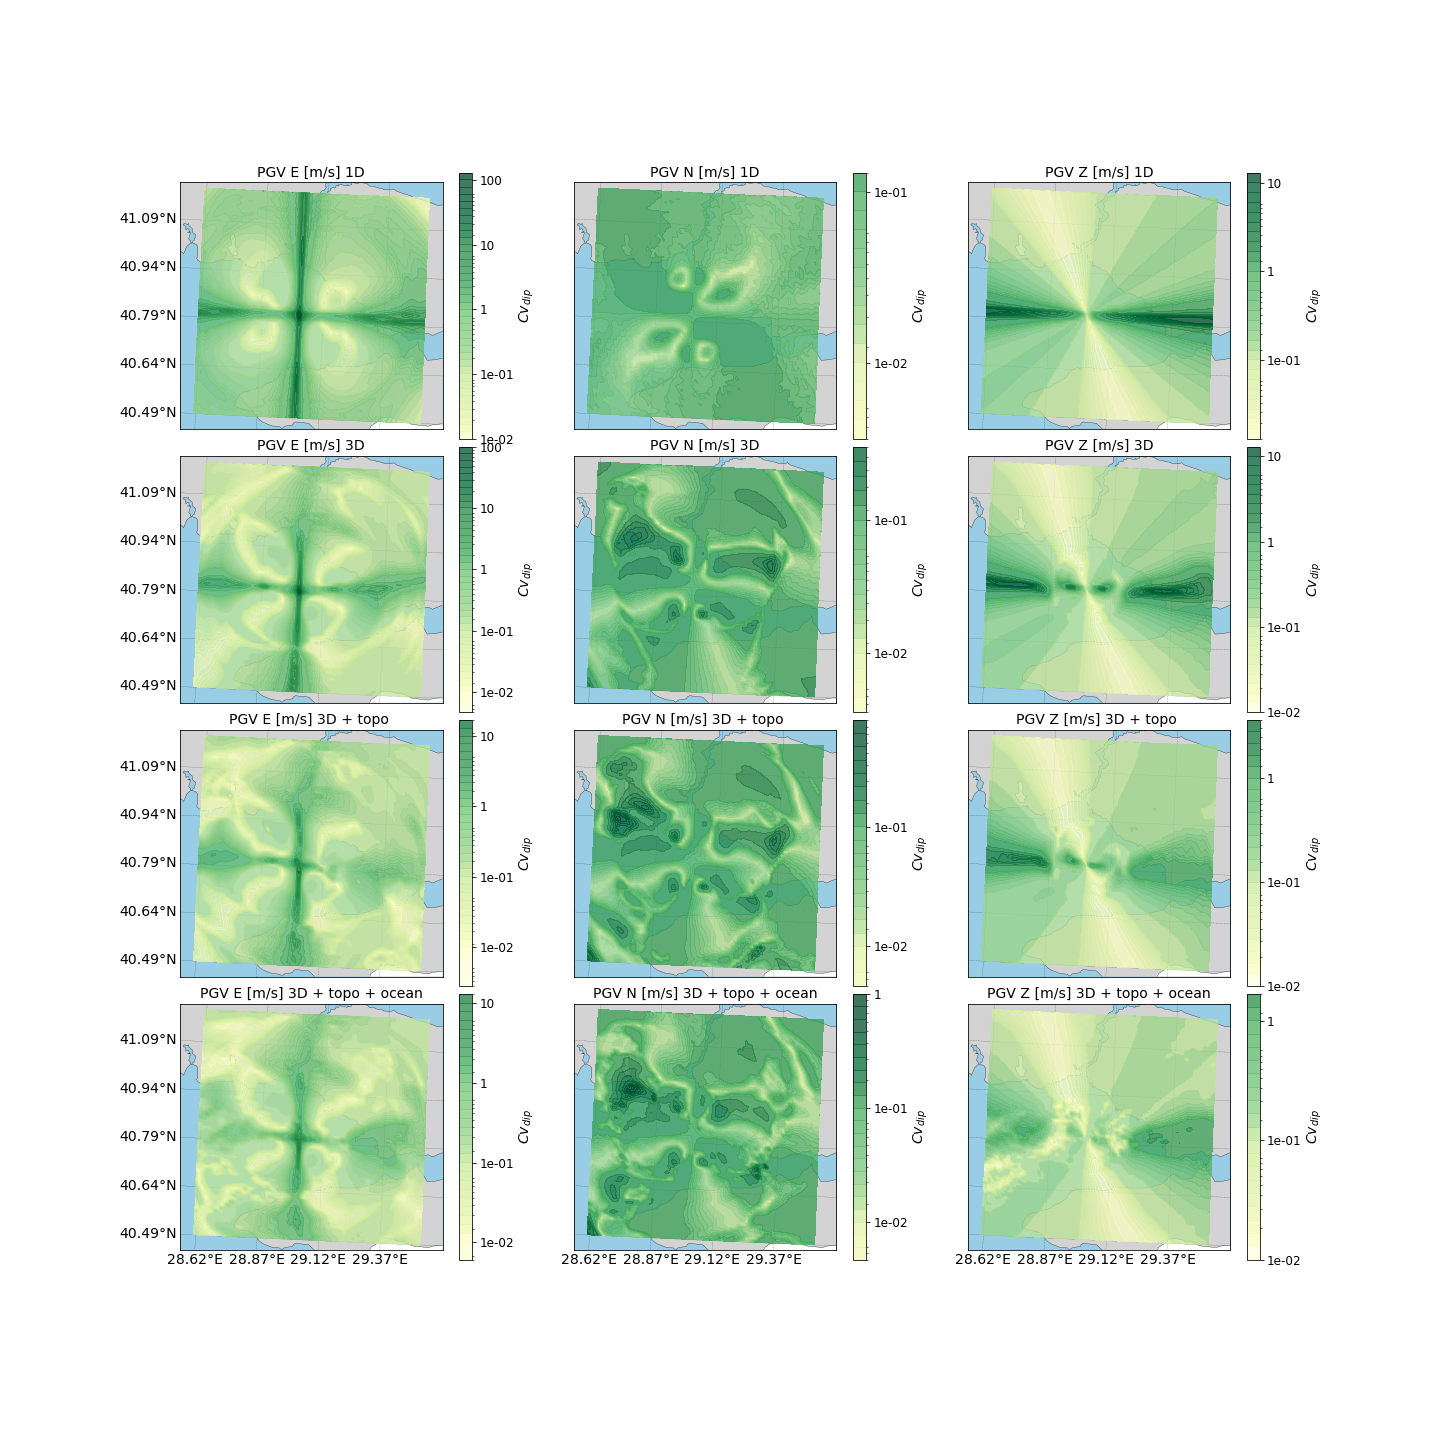
\includegraphics[width=1.2\linewidth]{images_results/dip_variation_sigma_sc1.png}
%     \caption{CMT1 coefficient of variation $Cv$ for dip, for each model domain in E, N and Z direction. Colourbar set to logarithmic to adequately show the large differences.}
%     \label{fig:ref_sigma1_dip}
% \end{figure}


% % check ff of dit klopt of het KAVV is



% \begin{figure}[H]
%     \centering
%     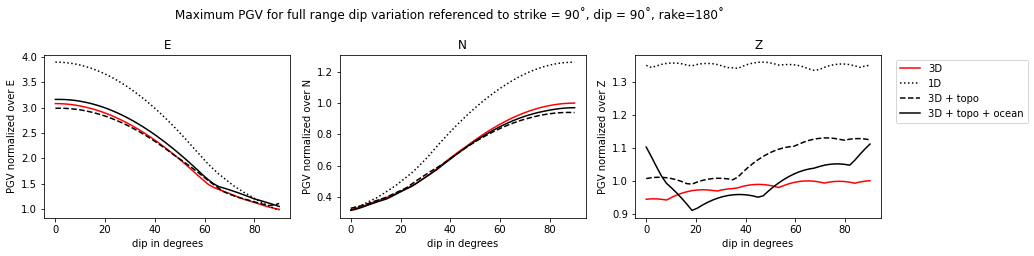
\includegraphics[width=0.8\textwidth]{images_results/fullrange1_dipvar_maxvals.png}
%     \caption{Full 180$\degree$ range variation of the strike measured at station KAVV.}
%     \label{fig:KAVV_fullrange_1_dip}
% \end{figure}


% \begin{figure}[h]
%     \centering
%     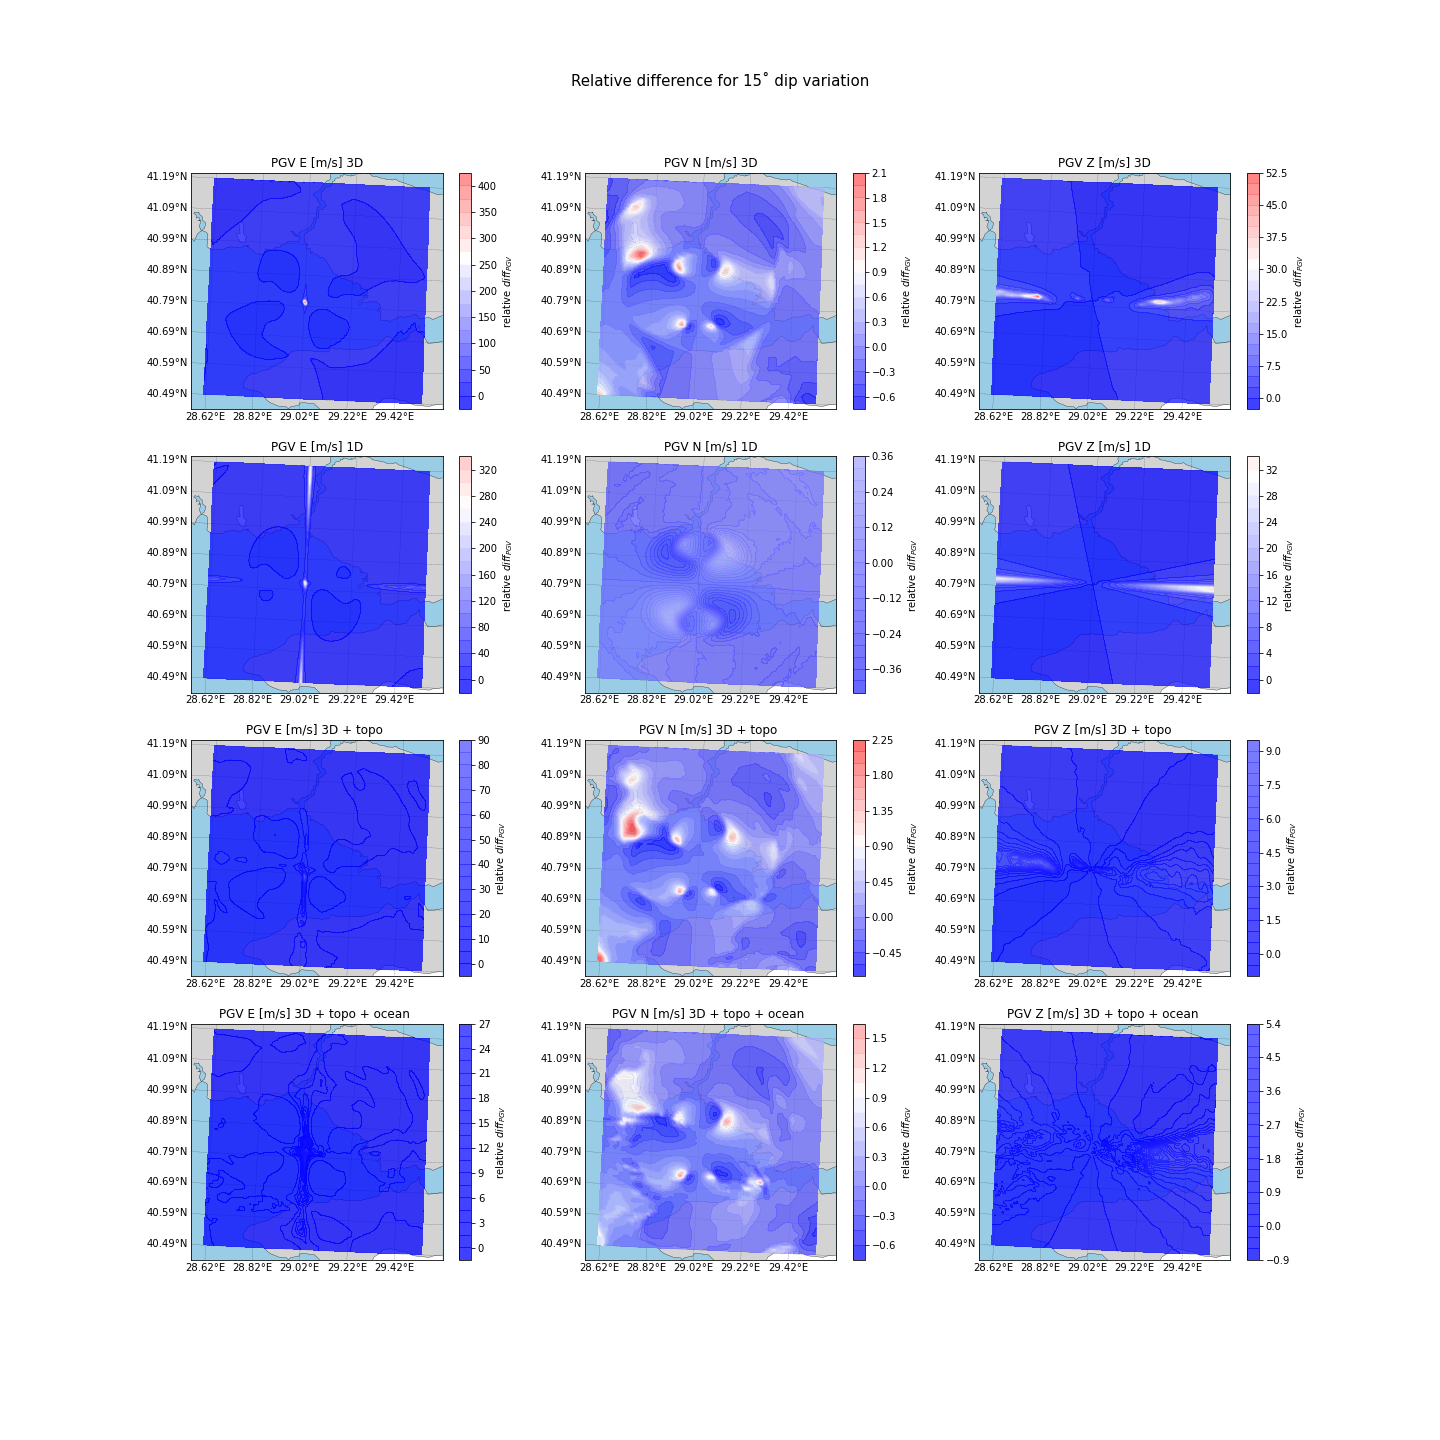
\includegraphics[width=1.2\linewidth]{images_results/dip_variation_epsilon12_sc1.png}
%     \caption{CMT1 relative difference between a scenario with a dip variation of 15$\degree$ with respect to the reference scenario. Colorbar set to the total minima and maxima of the 15$\degree$ and 25$\degree$ plots for comparison.}
%     \label{fig:ref_eps12-1_dip}
% \end{figure}

% \begin{figure}[h]
%     \centering
%     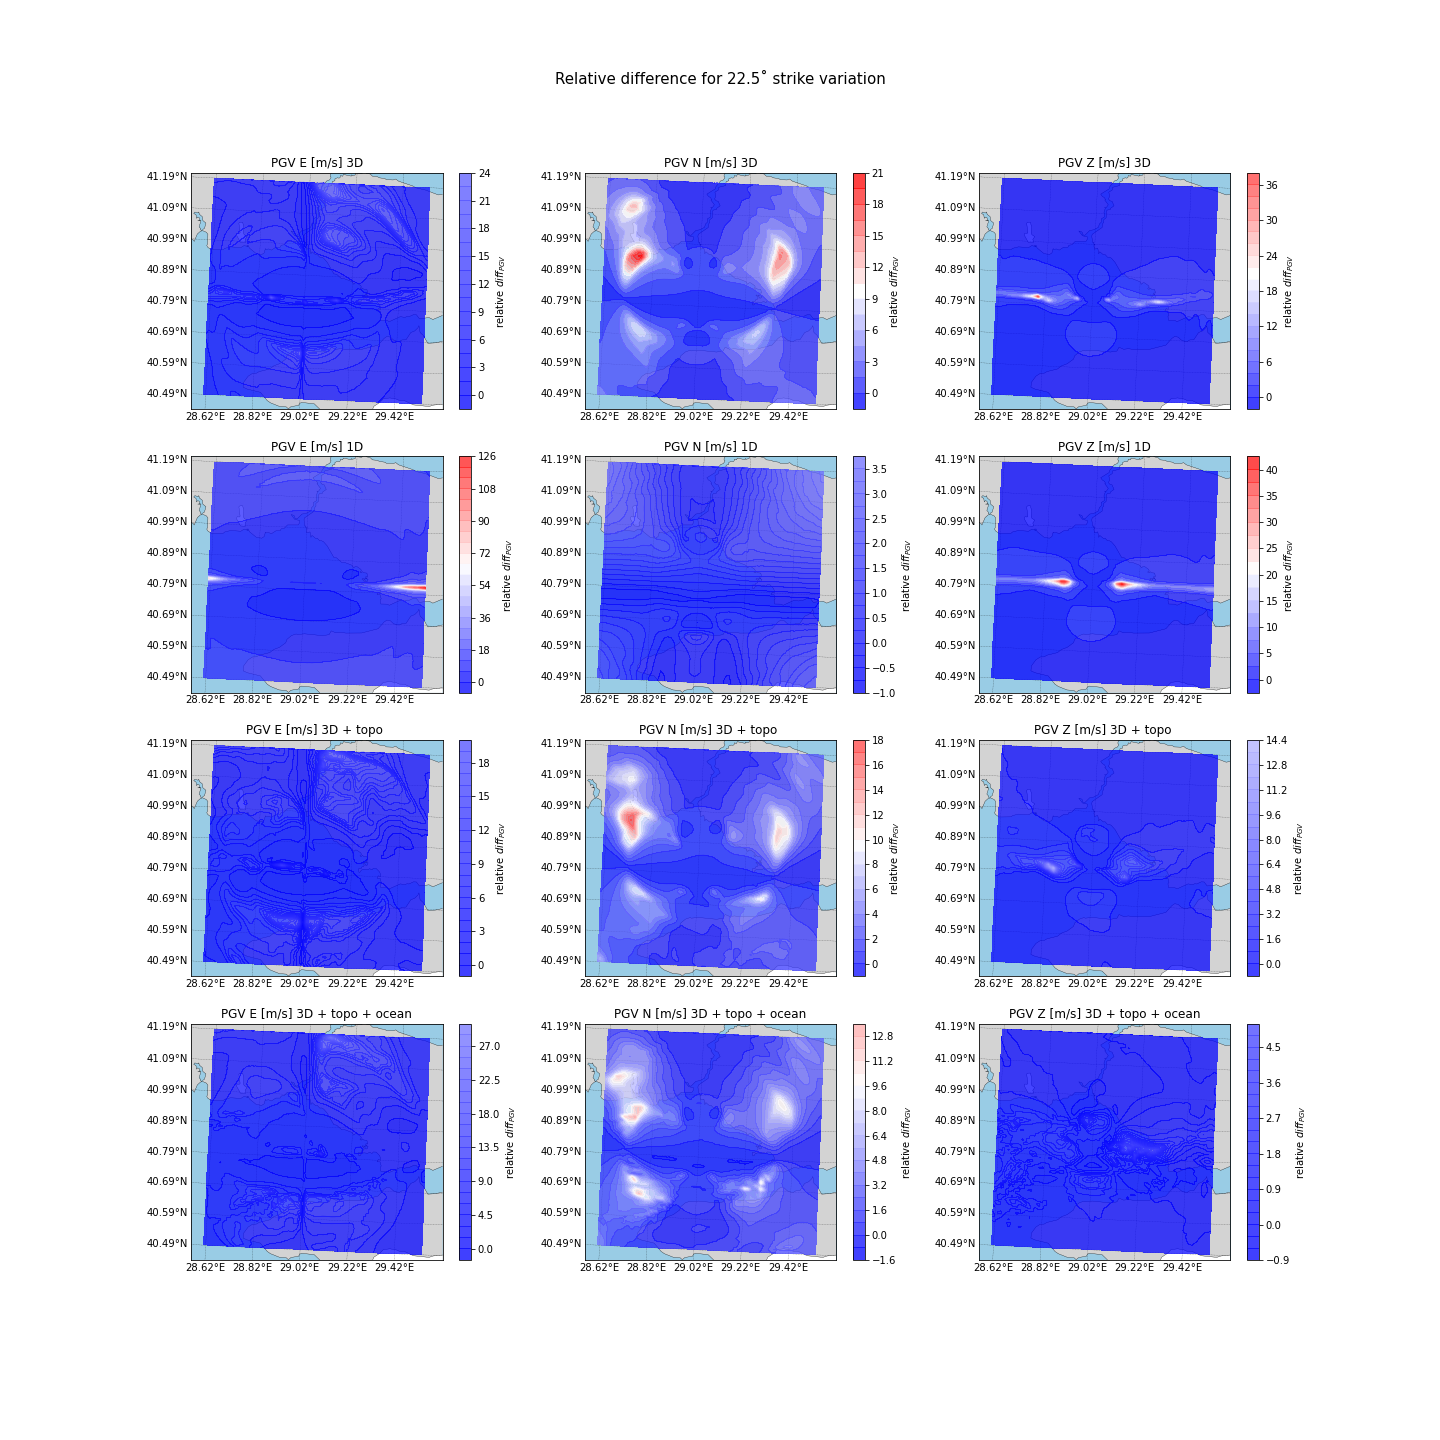
\includegraphics[width=1.2\linewidth]{images_results/strike_variation_epsilon25_sc1.png}
%     \caption{CMT1 relative difference between a scenario with a dip variation of 25$\degree$ with respect to the reference scenario. Colorbar set to the total minima and maxima of the 15$\degree$ and 25$\degree$ plots for comparison.}
%     \label{fig:ref_eps25-1_dip}
% \end{figure}



% \subsubsection{CMT 2}



% \begin{figure}[h]
%     \centering
%     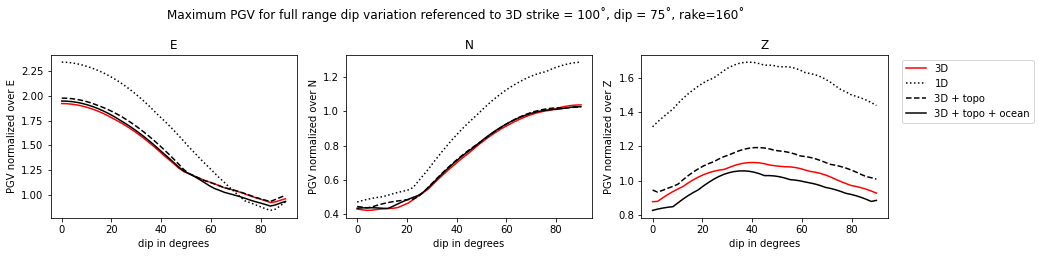
\includegraphics[width=0.8\textwidth]{images_results/fullrange2_dipvar_maxvals_sc2.png}
%     \caption{CMT2 Full 180$\degree$ range variation of the dip measured at station KAVV.}
%     \label{fig:KAVV_fullrange_2_dip}
% \end{figure}


% \begin{figure}
%     \centering
%     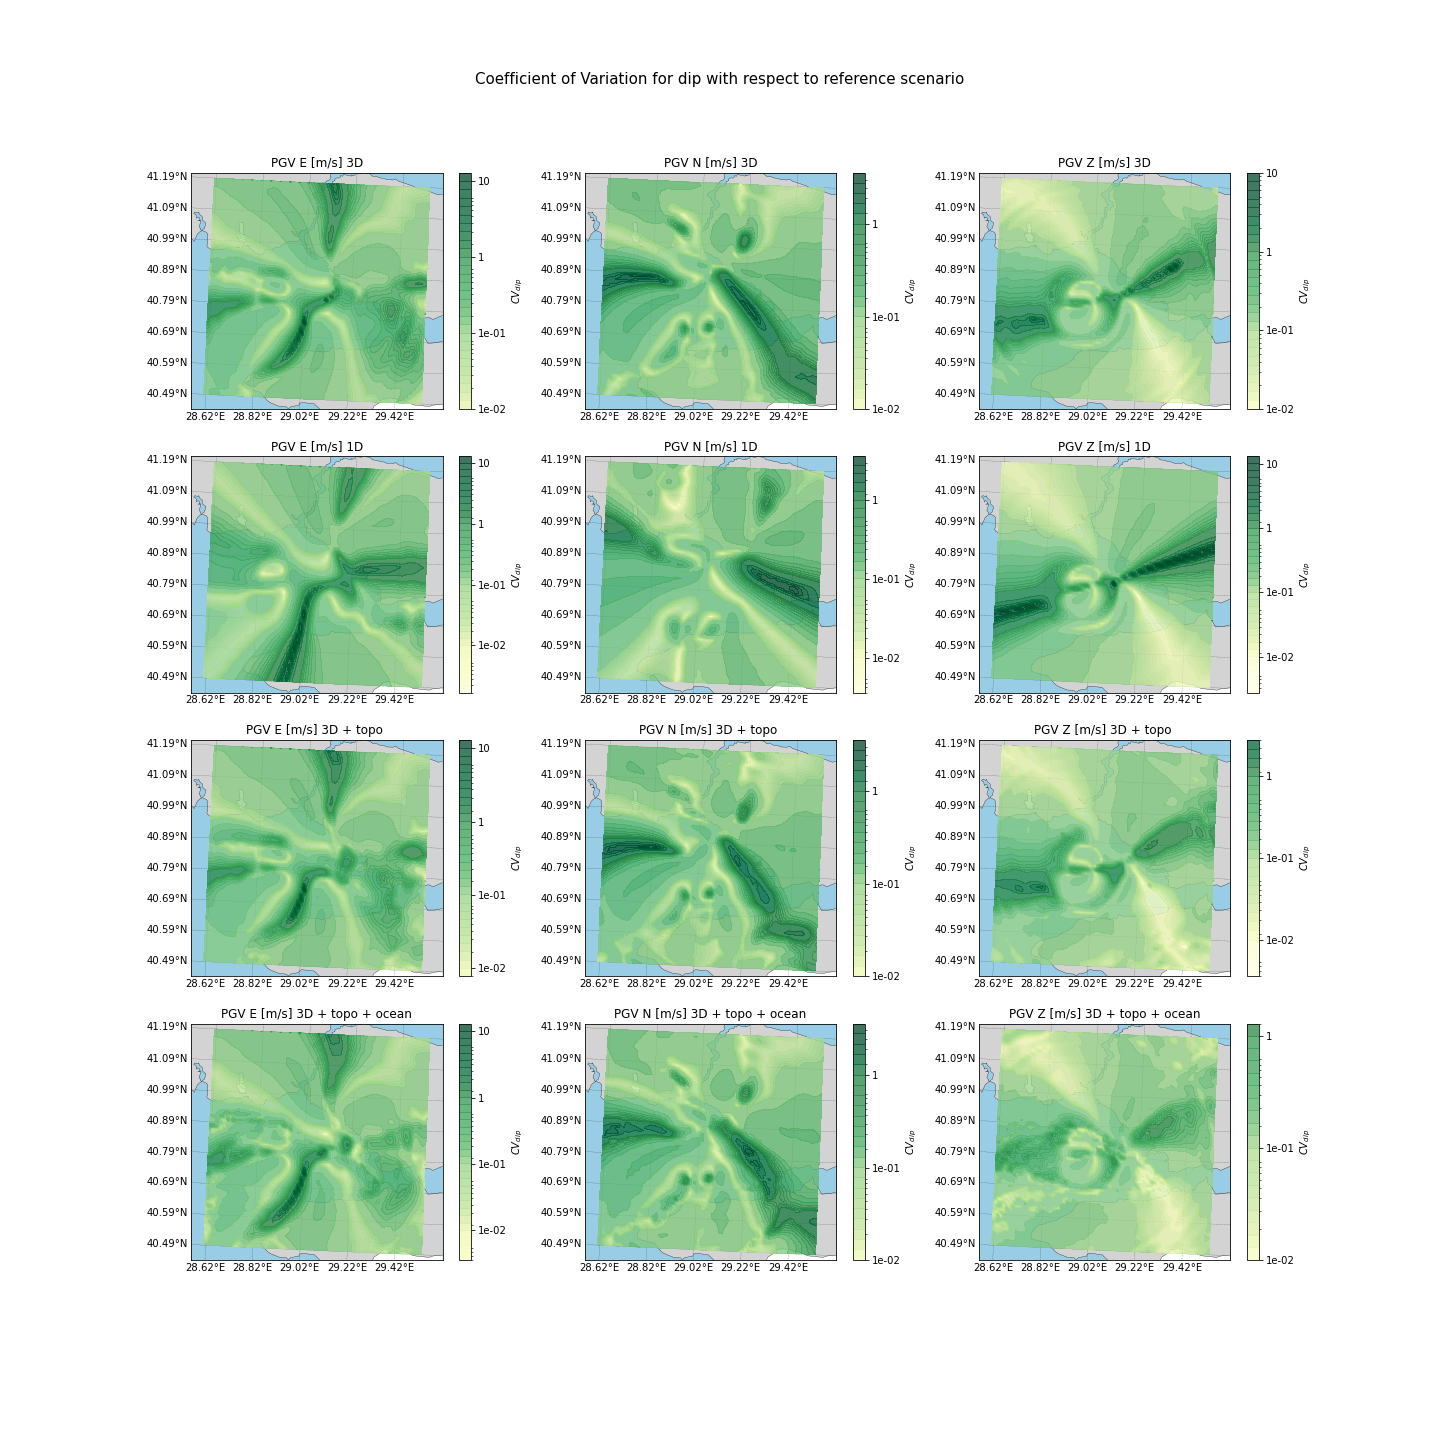
\includegraphics[width=1.2\linewidth]{images_results/dip_variation_sigma_sc2.png}
%     \caption{CMT2 coefficient of variation $Cv$ of dip variation, for each model domain in E, N and Z direction. Colourbar set to logarithmic to adequately show the large differences.}
%     \label{fig:cmt2sigm}
% \end{figure}



% \begin{figure}
%     \centering
%     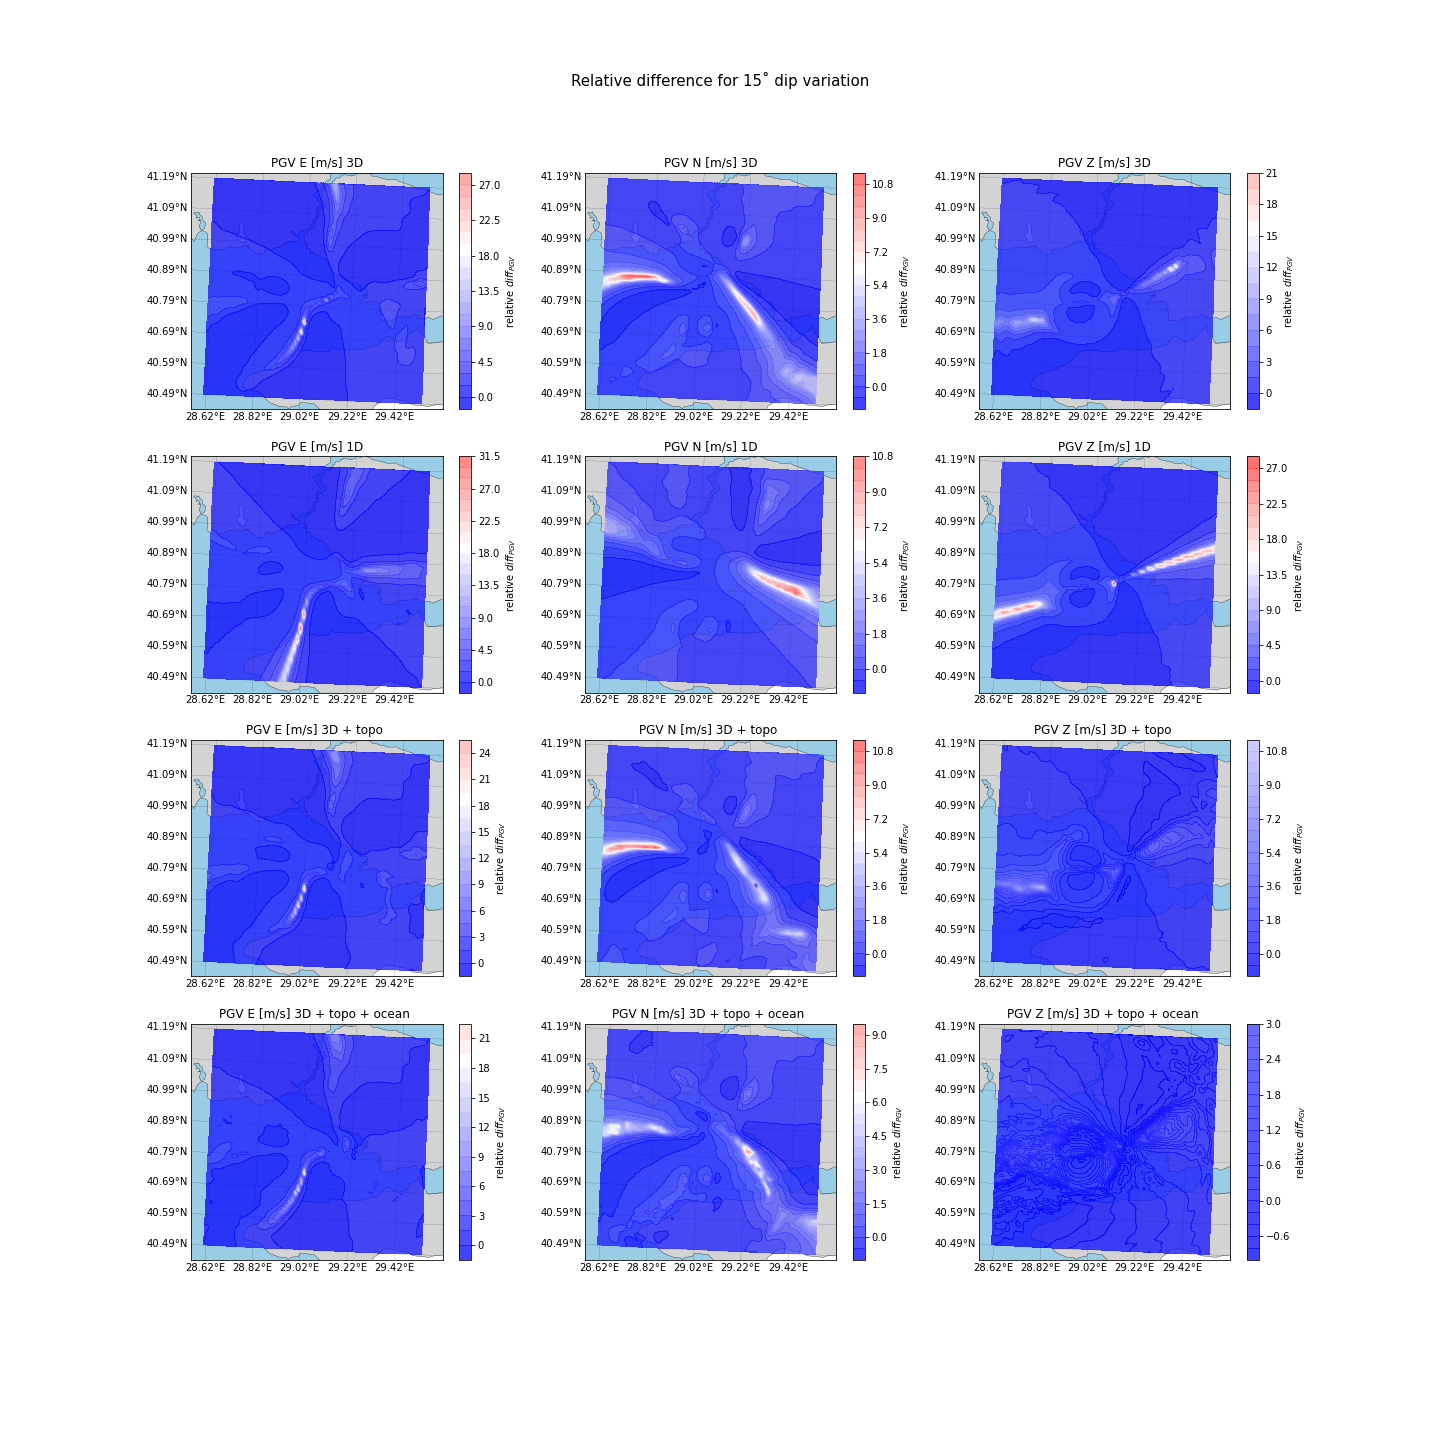
\includegraphics[width=1.2\linewidth]{images_results/dip_variation_epsilon12_sc2.png}
%     \caption{CMT2 relative difference between a scenario with a dip variation of 15$\degree$ with respect to the reference scenario. Colorbar set to the total minima and maxima of the 15$\degree$ and 25$\degree$ plots for comparison.}
%     \label{fig:ref_eps12-2}
% \end{figure}

% \begin{figure}
%     \centering
%     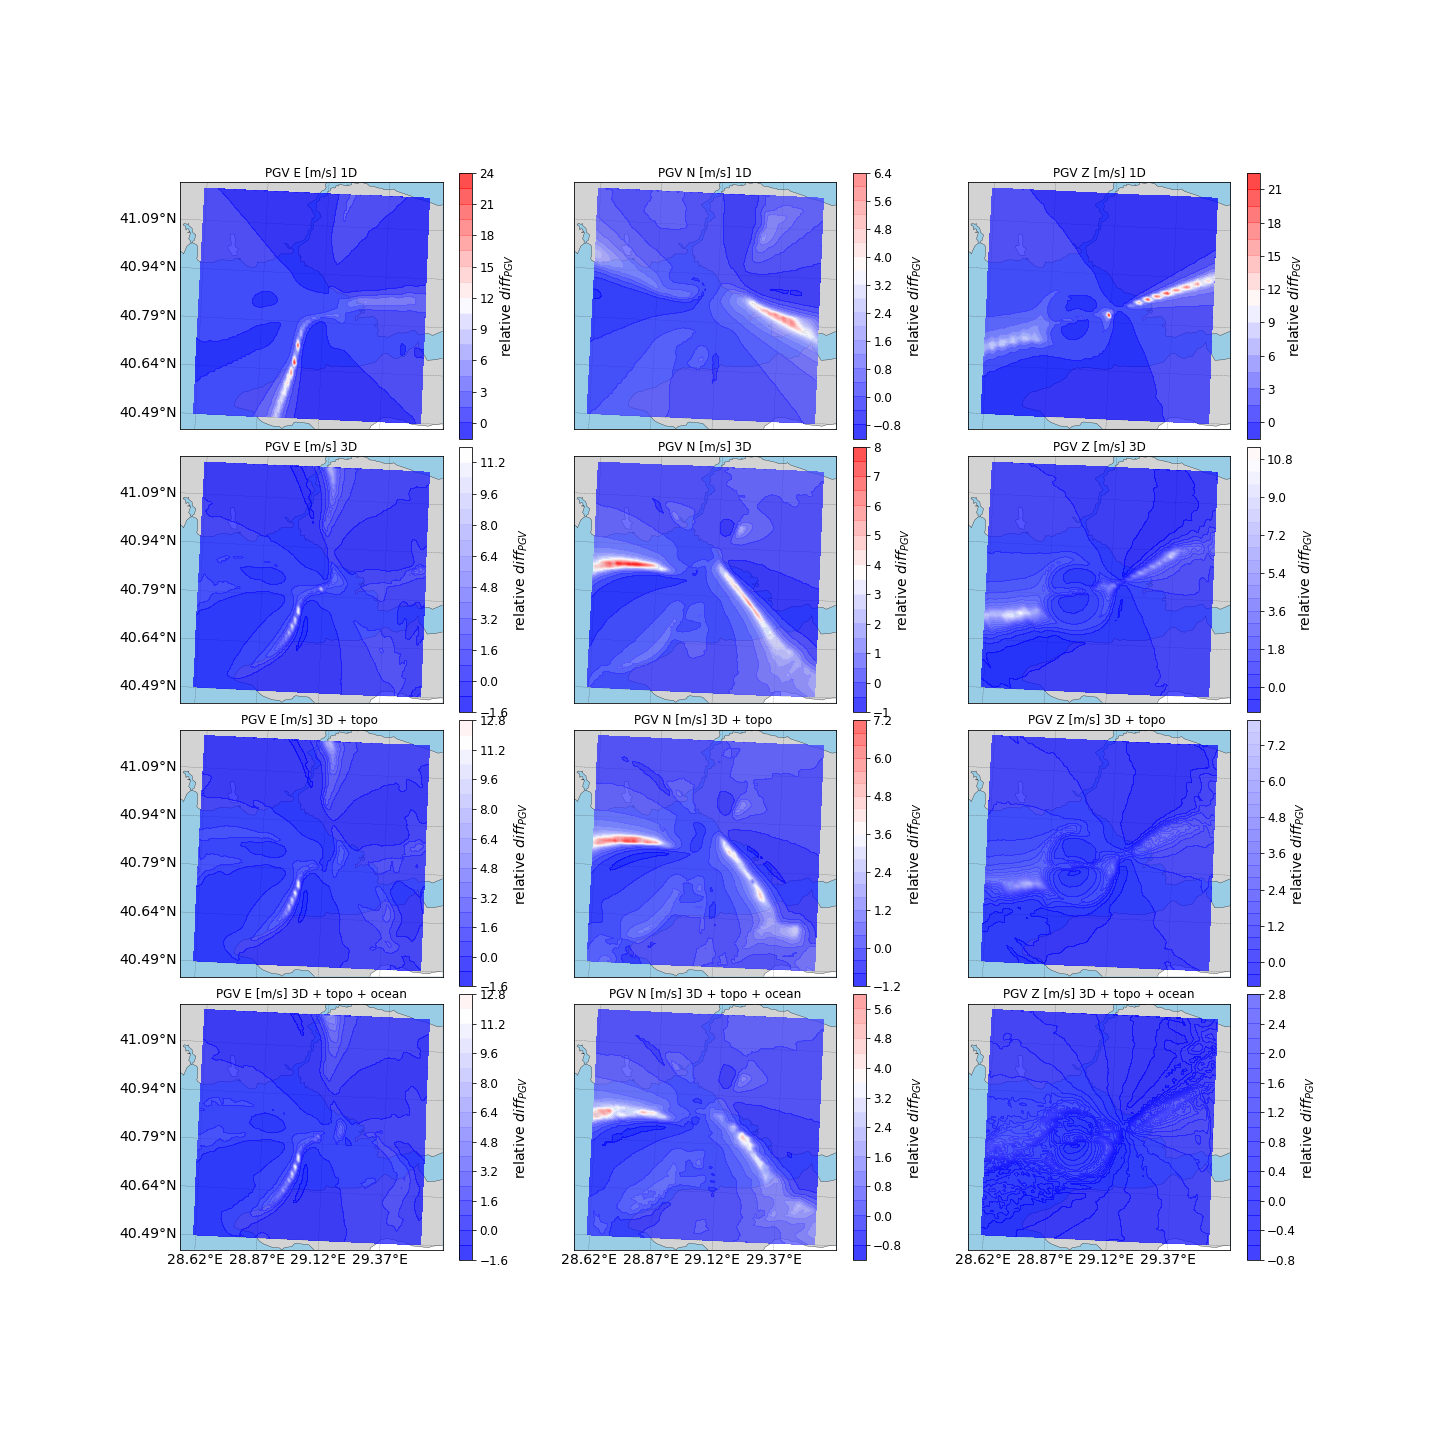
\includegraphics[width=1.2\linewidth]{images_results/dip_variation_epsilon25_sc2.png}
%     \caption{CMT2 relative difference between a scenario with a strike variation of 25$\degree$ with respect to the reference scenario. Colorbar set to the total minima and maxima of the 15$\degree$ and 25$\degree$ plots for comparison.}
%     \label{fig:ref_eps25-2}
% \end{figure}


\subsection{rake}














%%%%%%%%%%%%%%%%%%%%%%%%%%%%%%

\section{Source depth and location}

\hl{To do: show how shifting the location of the source mostly shifts the pattern with that amount meters at this scale. Show the variation of depth and its effects on PGV in the different domains}

[location variation standard deviation PGV]

[Depth variation standard deviation PGV]

\begin{itemize}
    \item Show that location shifts the signal mostly
    \item Show impact of depth variations
\end{itemize}

\section{Source time function}

\hl{To do: image of difference in patterns when a custom Ricker wavelet is used as source-time function. Just model this for one moment tensor in a domain with topography and ocean.}


\section{Short case study of a $M_w 7.0$ earthquake}

Although a CMT source representation is not an accurate approximation for earthquakes of $> Mw ??$, it is the type of source that can be inverted for directly after the event has occurred. As discussed earlier in section \hl{section}, it is the first step in the proposed urgent workflow of ChEESE  before a dynamic kinematic rupture scenario is simulated. To put the relative values of the previous sections into a practical perspective, we shortly assume a $M_w 7.0$ earthquake scenario at with the location, depth and nodal plane at CMT2. 

\hl{To do: Just to give some context to the relative cases of before, show a map with actual PGV values and the amount of standard deviation from this in the context of this scenario. Also show records at the three stations of this event.}

%[image 1D E, N, Z real values PGV, PGA , Arias]

%[image 3D E, N, Z real values + difference to 1D PGV, Arias]

%[image 3D + topo E, N, Z real values + difference to 3D PGV, Arias]

%[image 3D + topo  \& Ocean E, N, Z real values + difference to 3D + topo PGV, Arias]

%[image Spectral response on 3 real station locations]

\begin{itemize}
    \item comment on changes in pattern of the real values 
    \item comment on ground shaking of this scenario
\end{itemize}








\end{document}